\documentclass[sigplan,10pt,review,anonymous]{acmart}
\settopmatter{printfolios=true,printccs=false,printacmref=false}

% Packages {{{
\usepackage{amsmath}
\usepackage{amssymb}
\usepackage{tikz}
\usetikzlibrary{calc}
\usetikzlibrary{graphs}
\usetikzlibrary{cd}
\usepackage{bussproofs}
\usepackage{stmaryrd}
\usepackage{calc}
\usepackage{bbm}
% }}}

% Macros {{{

\newcommand{\kw}[1]{\ensuremath{ \textsf{#1} }}
\newcommand{\ifr}[1]{\ [{#1}]\ }
\newcommand{\ifrw}[2]{\ [{#1}]_{#2}\ }
\newcommand{\alt}{\ |\ }

\newcommand{\EC}{\kw{C}}
\newcommand{\simrel}{\kw{simrel}}

% Moves
\newcommand{\mcall}[3]{\kw{#1}({#2})@{#3}}
\newcommand{\pcall}[3]{%
  \underline{\mcall{#1}{#2}{#3}}%
}
\newcommand{\mret}[2]{{#1}@{#2}}
\newcommand{\pret}[2]{%
  \underline{\mret{#1}{#2}}%
}
\newcommand{\mretx}[3]{{#1}@{#2}/{#3}}
\newcommand{\pretx}[3]{%
  \underline{\mretx{#1}{#2}{#3}}%
}

% Pointers for justified sequences %{{{

% Parameters
\newcommand{\pshift}{1.6ex}
\newcommand{\pcdist}{2.5}
\newcommand{\pcangle}{60}

% Pointer hook
\newcommand{\ph}[1]{%
  \tikz[remember picture]{\coordinate (#1);}}

% Pointer to
\newcommand{\pt}[1]{%
  \rule{0pt}{1.4em}%
  \tikz[remember picture, overlay]{
    \draw[->]
      let \p{dest} = (#1),
          \n1 = {ln(veclen(\x{dest}, \y{dest}) + 1)},
          \p1 = ($(0,0)+(0,\pshift)$),
          \p4 = ($(#1)+(0,\pshift)$),
          \p2 = ($(\p1)!\n1*\pcdist!-\pcangle:(\p4)$),
          \p3 = ($(\p4)!\n1*\pcdist!+\pcangle:(\p1)$) in
        (\p1) .. controls (\p2) and (\p3) .. (\p4);}}

%}}}

% }}}

% Various parameters {{{
\bibliographystyle{ACM-Reference-Format}
\citestyle{acmnumeric}
%}}}

\begin{document}

\title{%
  The Essence of Deep Specifications
}

\author{J\'er\'emie Koenig}
\affiliation{
  \department{Computer Science}
  \institution{Yale University}
}
\email{jeremie.koenig@yale.edu}

\begin{abstract} %{{{
\end{abstract}
%}}}

\maketitle

\section{Introduction}

In recent years,
formal verification of computer systems
of increasing size has become practical.
Researchers have been able to verify complex artifacts
at a variety of abstraction levels spanning
from CPU designs to network protocols.

These achievements remain discrete efforts, but
there has been increasing interest in rendering them interoperable,
as exemplified by the DeepSpec project.
The ability to connect correctness proofs of components
verified at various levels of abstraction
would enable the construction of extremely reliable heterogenous systems
through end-to-end verification.

In this paper,
we propose that a successful synthesis of existing research on
game semantics,
refinement-based methods,
abstraction layers and
logical relations
has the potential to serve as a common theory
of certified components.

\subsection{Game semantics} %{{{

The mathematical study of the semantics of programming languages
has traditionally opposed denotational and operational approaches.
Operational semantics describes
the behavior of a program in terms of
a state evolving across time.
Denotational semantics is a more abstract approach,
whereby the meaning of a program fragment (its denotation)
is computed from the meanings of its constituents.

This compositionality makes denotational semantics
more amenable to some forms of large-scale reasoning,
but its abstract character makes it more difficult
to connect to the concrete behavior of the system.
Therefore, when defining a denotational semantics,
it is customary to demonstrate its accuracy
with respect to an operational model.
This is done by proving a full abstraction theorem,
which asserts that the denotations of two programs
are equal exactly when the programs are observationally equivalent.

Game semantics is a denotational approach that
incoroporates some operational aspects.
Each type in the language
is interpreted as a game,
which specifies the structure of the interaction
between program components of this type
and their execution context.
The behavior of a component
is then modeled as a strategy for this game,
specifying the next move of the component
for all relevant positions in the game.

Positions are usually identified with sequences of moves,
and strategies can be identified with the set of positions
that a component can reach.
In this sense,
game semantics is similar to
the trace semantics of process algebras.
However, game semantics is distinguished
by a strong polarization between
the system and the environment,
and a strong distinction between outputs and inputs.
This confers an inherent ``rely-guarantee'' flavor
to games which facilitates compositional reasoning
in the context of heterogenous systems \cite{cspgs}.

%}}}

\subsection{Refinement-based verification} %{{{

The goal of program verification
is to establish that a program conforms
to a given mathematical specification.
In refinement-based approaches,
programs and specifications are interpreted in the same
semantic domain,
and conformance is expressed in terms of a
refinement preorder.

In stepwise refinement methods,
programs and specifications share a common syntax as well,
and the program is derived
by making the specification progressively more concrete,
ensuring that refinement holds at each step:
\[ \llbracket P \rrbracket \sqsubseteq
   \llbracket S_n \rrbracket \sqsubseteq
   \cdots \sqsubseteq
   \llbracket S_1 \rrbracket \sqsubseteq
   \llbracket S \rrbracket \]
By contrast,
we will use the elements of the semantic domain
directly as our specifications,
so that conformance will be expressed as:
\[ \llbracket P \rrbracket \sqsubseteq \sigma \,. \]

Refinement is commonly used in operational models,
for instance in the form of simulations
for labeled transition systems.
Denotational semantics also make extensive use of
orders on the semantics domain,
in particular in its treatment of recursion and divergence.

However,
the information orderings traditionally used
in the context of denotational semantics
are not appropriate as a notion of refinement,
because they regard silent divergence
as the absence of information ($\bot$).
In the context of verification,
we need to consider silent divergence
as a behavior on par with others,
or at the very least as a catastrophic failure
that can only implements itself ($\top$).

[Should mention contextual refinement]

[In Sec. X we distance from abstract, fixpoint treatment
of divergence and choose a more operational treatment
more in line with CCS and the like.]

%}}}

\subsection{Logical relations} %{{{

In the broadest sense,
logical relations are structure-preserving relations,
in the same way that homomorphisms are structure-preserving maps.
However,
logical relations are more compositional than homomorphisms,
because they do not suffer from the same problems
in the presence of mixed-variance constructions,
such as the function arrow $\rightarrow$ \cite{lrp}.
This is a major advantage
for reasoning about typed languages,
where type-indexed logical relations
can be defined by recursion over the structure of types.

Logical relations have found widespread use in programming language theory.
Unary logical relations can be used to establish
various properties of type systems:
a type-indexed predicate expressing a property of interest
is shown to be compatible with the language's reduction,
and to contain all of the well-typed terms of the language.
Binary logical relations can be used to capture
contextual equivalence between terms,
as well as notions such as non-interference or compiler correctness.
Relational models of type quantification yield
Reynold's well-known theory of relational parametricity,
and can be used to establish so-called free theorems
establishing properties that
all terms of a given parametric type must satisfy.

For stateful languages,
which terms should be related
will often depend on the current state.
This motivated the introduction of Kripke logical relations,
which are parametrized over a set of state-dependent \emph{worlds}.
Different components related at the same world
will be guaranteed to be related in compatible ways.
An accessibility relation between worlds
specifies the ways in which a world can evolve
as the execution progresses.

In Sec.~\ref{sec:klr},
we give a general account of Kripke logical relations
by drawing on their connection with
the Kripke semantics of modal logic.
We apply this framework
in our treatment of refinement
in the context of game semantics,
and in Sec.~\ref{sec:cklr},
we use it to develop a logical-relations
understanding of some key aspects of CompCert,
and show how parametricity
can be used to derive important properties
of CompCert languages.

Logical relations can be of any arity,
but in the present work
we will restrict our attention to
binary logical relations.

%}}}

\subsection{Abstraction layers} %{{{

%}}}

\subsection{Compilers} %{{{

Compilers play a central role
in the construction of modern computer systems.
A compiler is the quintessential tool
in bridging abstraction layers ---
and its calling convention
the quintessential expression of their relationship.
[Mention how CertiKOS is framed as a certified compiler.]
As such,
any methodology seeking to scale up
the construction of certified systems
must convincingly account for compilation
as a central principle.

Since the introduction of the fomally verified
Compcert C compiler a decade ago \cite{compcert},
there have been very successful efforts aimed at
interfacing it with other verification tools (VST),
using it as a component in larger verification projects (CertiKOS),
and refining its correctness theorem
to model real-world compiler use
in increasingly realistic detail
\cite{qompcert,sepcompcert,compcompcert,compcerttso,compcertshm}.
With each step,
the user can gain more confidence in the reliability of Compcert:
existing work testing the correctness of existing compilers
has found fewer bugs in Compcert,
compared to unverified alternatives \cite{csmith},
and efforts to make Compcert's correctness theorem more realistic
have uncovered and removed some of the few remaining bugs \cite{sepcompcert}.

Yet, most of this work
focuses on the reliability of the compiler
as an individual component.
The role this component plays in the construction of larger systems
is usually treated informally:
real-world use case scenarios are presented
to explain the meaning and justify the suitability
of the correctness theorem being proved.
However,
beyond \emph{system components that are certified},
achieving end-to-end verification of large-scale systems
will require \emph{components of certified systems},
which can in turn be used and composed
to build larger certified systems.

%}}}

\subsection{Contributions} %{{{

This article makes two significant contributions
towards a general framework for the construction of certified systems.

First, in Sec.~\ref{sec:rbgs} we introduce the general framework of
\emph{refinement-based game semantics}.
Like traditional game semantics,
refinement-based game semantics provides
a typed, compositional, semantic domain
supporting fully abstract expression of
the behavior of heterogenous components.
However,
by relaxing the traditional focus on definability,
our model can also express more general specifications,
and serve as a setting for refinement-based verification.
[enumerate some of the things we do]

Second, we demonstrate the suitability of our approach
by applying it to the problem of compositional certified compilation.
We show that we can build previous work \cite{compcomp,sepcomp,popl15,cpp15}
to equip CompCert with an open module semantics
that can naturally be embedded into our semantic framework.
Moreover,
our explicit account of abstraction
allows us considerable economy
when updating the correctness theorem of CompCert
to account for this additional structure,
and our logical-relations approach
makes it possible to ...

%}}}

\endinput

\subsection{Old stuff}

-----
The state of the art in formal verification is:
we can verify individual artefacts of decent size
(Compcert, CertiKOS, seL4, file systems, CPUs, network protocols).
But the grand challenge is figuring out
how to connect such components together
to obtain large-scale, end-to-end verified systems.
[name-drop the DeepSpec project, cyber-physical systems etc.]

In that context,
compilers are particularly interesting and relevant
because they are a ubiquitous tool
involved at many layers
in the construction of large-scale software systems.




To achieve this, we need to take
a more systematic view of
how large-scale systems are constructed and
how to reason about them,
and use that insight to
articulate design principles for
components of certified systems
and the mathematical tools we use to analyze them.

\subsection{[Innovation]}

In this work, we attempt to answer the question:
what is a \emph{composable} certified compiler?

We identify six criteria for theories of systems (ie. semantic domains)
to be suitable in the context of building larger systems:
expressivity, abstraction, refinement,
compositionality, open systems, resources.

We apply this analytical framework (or rather 1-5)
to the problem of certified compilation,
and to Compcert in particular.
Our criteria suggest natural,
minimal ways in which the semantic framework
used by Compcert should be extended.

We show that we can extend the correctness proof of Compcert
to fit this new framework and
demonstrate how the resulting artefact
can be used to construct fancy certified stuff.

Our analytical framework is also a good way to:
evaluate the limitations of our work
(we need more expressivity for concurrency,
we don't have a good story for resources);
classify and compare previous work on compositional compilation;
map out promising directions for future work.

{\color{gray} %{{{

\subsection{Obsolete ramblings}

[XXX: Redistribute into the main ideas section]

Challenges:
\begin{enumerate}
\item Expressivity.
  [Need not be achieved all at once,
  if we can embed the semantic domain used to analyse a system
  into a broader one.
  The bar should be,
  our formalism should be rich enough to account for
  the full range of possible interaction of a system with its environment
  in the real world.
  Then there should be a way to embed in the formalism
  used to analyze / build any larger system of which it is a component.
  We demonstrate this when we build our richer semantics of Compcert in Sec~4
  and embed our minimalistic one from Sec~3.]
\item Compositionality.
  [Complex systems can only be understood
  as the relationship of simpler components,
  which can be reasoned about in isolation.]
\item Open systems.
  [Compositionality should work from the bottom up, not top down.
  Components should not be understood as fragments of a fixed whole.
  There is no whole system.
  Every system is a component.
  \emph{But},
  it may be reasonable to partially close a subsystem
  after we built it up from components,
  as long as the resulting one
  is still able to interact with its environment]
\item Abstraction.
  [Reductionism is shit.
  You can't \emph{understand} a book
  as a collection of atoms of ink, paper and glue.
  Let alone how that relates to the corresponding e-book.
  Let alone its place within a genre of literature.
  Every level of abstraction exists in its own right.
  Its nature cannot be explained by a particular realization.
  The relation between them ]
\item Refinement.
  [The role of a component is realized in a specific way.
  We don't want to sweat the details when looking at the big picture.]
\item Resources.
  [The role of a component is realized in an imperfect way.
  An ideal, infinite model only exists in the real world
  as a series of finite approximations;
  resource limitations introduce a discontinuity.
  Abstractions break down beyond certain threshold:
  we run out of stack space,
  insufficient network capacity introduces congestion,
  a heap becomes too fragmented to satisfy
  requests for a contiguous block of memory.

  A satisfactory treatment of resources
  allows us to caracterize the range of conditions
  under which refinement and abstraction hold,
\end{enumerate}

In the context of the theory programming languages,
[enumerate things that have tackled combinations of these
challenges:
subtyping -> refinement;
traditional game semantics -> expressivity, compositionality, open systems;
interface automata -> compositionality, $\approx$ open systems, refinement;
certikos -> abstraction, refinement;
lax modality -> compositionality, resources;
logical relations -> abstraction and refinement (sometimes), compositionality;
...]

Context of Compcert:
original compcert uses relatively expressive model
(event traces are fairly general),
and has a notion of refinement (inclusion of sets of behaviors, Vundef),
but not compositional (whole program),
not that open (it's unclear how to connect all kinds of interesting things),
no abstraction (behavior of source and target expressed in same model),
no account of resources (infinite stack at Asm).

[mention that Compcert's model of the userspace is very naive;
impossible to encode a specification such as POSIX
as external function semantics]

Various works seek to extend to support some of these things:
CompCompCert, separate compcert, CompCertX, Qompcert

In this paper:
sketch something for challenges 2-5
out of (traditional game semantics + interface automata + abstraction layers).
Illustrate how these ideas play out in the context of compilers,
and apply them to solve the open problem of
compositional certified compilation.

\subsection{Contributions}

Specifically,
we identify six principles [...]
Give a clear ``test'' for each.
Can guide design.

We apply our analytical framework to the problem of certified compilation:
\begin{itemize}
\item analyze previous work in pl semantics and certified compilation
  in this framework to assess and explain the strenghts and weaknesses of each
  [sec. 12 Related Work]
\item show [in sec. 3 Semantics with External Calls]
  how these ideas yield a natural solution
  when applied to the open problem of compositional compilation
\item formulate new challenge / next step:
  that of a compiler which can be used as a component
  for end-to-end verification;
\item In Sec.~4 [richer semantics],
  show that our semantic model can be made more expressive
  in a way that our compiler remains correct in that setting;
\item In Sec.~5 [applications],
  illustrate with some applications
  the ways in which our compiler can be connected
  to a larger system
\item Assess the remaining gap between our compiler
  and our new challenge (concurrency, resources),
  and apply our analytical framework to suggest
  what a solution might look like.
\end{itemize}

[Basic claim: the answer to compositional verification
is an undestanding of abstraction and refinement in the context of games.]
The present work applies this analysis to
solve the open problem of certified compositional compilation of low-level languages
plus an understanding of refinement and abstraction in that context.]

\subsection{Limitations}

No concurrency
(not expressive enough:
accesses to memory between external calls are not observable
--- this being said existing work on Concurrent CertiKOS shows
it may be possible to map our model in a more general one),
no good story for resources.

In Sec.~N [Future Work] [spell out some leads to fill these gaps.]

} %}}}

\section{Main ideas}

\subsection{Principles for system construction}

The goal of certified system design is
to create a formal description of
the system to be constructed (the program),
while ensuring through careful analysis that the system
will behave properly.

To carry out this analysis,
we need a model
which assigns to each possible system description $p \in P$
a mathematical object $\llbracket p \rrbracket \in \mathbb{D}$
representing its behavior.
We will call the set $\mathbb{D}$ a \emph{semantic domain}.
In this section we elucidate
the structure and properties of $\mathbb{D}$
necessary to the process of builing
large-scale certified systems.

\paragraph{Specifications and refinement}

System design starts with a set of requirements
that constrain the behavior of the system to be constructed
(the specification).
These requirements may not capture every detail
of the behavior of the eventual system,
but instead delineate the range of acceptable behaviors
from the point of view of its environment.

In the context of refinement-based methods,
the specifications are themselves elements of
the semantic domain $\mathbb{D}$,
which is equipped with a \emph{refinement} preorder
${\sqsubseteq} \subseteq \mathbb{D} \times \mathbb{D}$.
The proposition $\sigma_1 \sqsubseteq \sigma_2$
assert that $\sigma_2$ is a less restrictive specification than $\sigma_1$,
and in particular a system description $p \in P$ is a correct implementation
of $\sigma \in \mathbb{D}$ when:
\[ \llbracket p \rrbracket \sqsubseteq \sigma \]

\paragraph{Compositionality}

Complex systems are built by assembling components
whose behavior is understood,
such that their interaction achieves a desired effect.
The syntactic constructions of
the language used to describe systems
correspond to the ways in which they can be composed.

To enable compositional reasoning,
a suitable model must provide an account of
the behavior of the composite system
in terms of the behavior of its parts.
For instance,
if the language contains a binary operator
${+} : P \times P \rightarrow P$,
then the semantic domain should be equipped with
a corresponding operation
${\bullet} : \mathbb{D} \times \mathbb{D} \rightarrow \mathbb{D}$
such that:
\[ \llbracket p_1 + p_2 \rrbracket =
   \llbracket p_1 \rrbracket \bullet \llbracket p_2 \rrbracket \,. \]

We can use this property
to show that a composite system
satisfies a given specification,
for instance
$\llbracket p_1 + p_2 \rrbracket \sqsubseteq \sigma$.
Once this has been established,
we will want to abstract the composite system as a ``black box''
which can in turn be used as a primitive component in a larger system.
Further reasoning can be done in terms of
the new component's specification $\sigma$ rather than
its concrete behavior $\llbracket p_1 + p_2 \rrbracket$.
To support this,
we must establish that semantic composition operators
are compatible with refinement in the following sense:
\[ \sigma_1 \sqsubseteq \sigma_1' \wedge
   \sigma_2 \sqsubseteq \sigma_2' \Rightarrow
   \sigma_1 \bullet \sigma_2 \sqsubseteq \sigma_1' \bullet \sigma_2' \,. \]
Should $p_1 + p_2$ be used as a component in a larger system,
this property will allow us to establish that:
\[ \llbracket (p_1 + p_2) + p_3 \rrbracket \sqsubseteq
   \sigma \bullet \llbracket p_3 \rrbracket \,. \]

\paragraph{Abstraction}

Large-scale systems operate across many layers of abstraction.
Each abstraction layer defines its own ``view'' of the interaction
between the system and its environment:
at the physical level,
communication over a wire may involve a series of voltages through time,
but at a higher level of abstraction
we will only be concerned with the sequence of bytes
being transmitted.

The correspondance between the two can be expressed as an embedding
$\mathbb{C} : \mathbb{D}_s \rightarrow \mathbb{D}_t$
between the semantic domains
used to reason at different levels of abstraction.


Serial communication hardware (for instance a UART device)
serves as a bridge between these two views,
implementing a byte-oriented communication channel
in a voltage-oriented world;
to formally verify such a component we will need to
express the correspondance between these two
layers of abstraction.




[...]

\paragraph{Compilers}


\paragraph{Heterogeneity}

[What happens to $\mathbb{D}$ in the context of typed languages,
how this can be used to gain expressivity and construct heterogenous systems.]


\subsection{Game semantics}

[introductory remarks]

Types are interpreted as two-player games,
which specify the form of valid interactions
between the system and the environment.
Terms are interpreted as strategies for these games,
which for any position in the game
specify the next move to be played by the system.

\paragraph{Games}

A game is usually defined by giving a set of moves $M$
that players can choose from,
as well as a specification of which
sequences of moves are considered valid.
For chess,
moves will be taken in the set $(\{a, \ldots, h\} \times \{1, \ldots, 8\})^2$,
and a sequence of moves may look like:
\[ e2e4 \cdot \underline{c7c5} \cdot c2c3 \cdot \underline{e7d5} \cdots \]
For a program expected to produce a natural number,
the possible moves may be a request to evaluate ($\kw{q}$)
and primitive values ($42$),
so that an interaction between the expression $21 \times 2 : \kw{nat}$
and its evaluation context will proceed as:
\[ \kw{q} \cdot \underline{42} \]
Note that we underline the moves of the second player,
namely the system.

We will focus on two-player, alternating games
where the environment and the system each contribute every other move.
The environment plays first.
Positions in the game can be given
as sequences of moves;
even-length sequences correpond to positions
where the environment is expected to move,
and odd-length sequences correspond to positions
where the system is expected to move.

\paragraph{Strategies}

In this context,
it is natural to think of system strategies
as functions from odd-length positions to moves:
\[ \sigma : \bigcup_n M^{2n+1} \rightharpoonup M \]
For example,
the strategy $\llbracket 21 \times 2 \rrbracket$
will be the partial function with a single mapping $\kw{q} \mapsto 21$,
whereas the black player in the chess play above
has used a strategy $\sigma$ containing:
\[
  \sigma(e2e4) = c7c5 , \quad
  \sigma(e2e4 \cdot c7c5 \cdot c2c3) = e7d5 , \quad
  \ldots
\]

This is suitable to express the behavior of a concrete system.
However, for specifications allowing a range of behavior,
we must generalize strategies to allow nondeterminism:
\[ \sigma : \bigcup_n M^{2n+1} \rightarrow \mathcal{P}(M) \]

Transition system:

\[ \sigma : \exists \, K S \,.\, K \times
      (K \times M \rightarrow \mathcal{P}(S)) \times
      (S \rightarrow \mathcal{P}(M \times K)) \]

\paragraph{Compositionality}

While the game for $\kw{nat}$ given above
is extremely simple,
the expressive power of game semantics
comes from the way in which complex games can be derived
from simple ones to interpret compound types.

For instance,
given two games $A$ and $B$,
the game $A \otimes B$ is traditionally defined
to allow $A$ and $B$ to be played side by side.
The set of moves will be $M_{A \otimes B} = M_A + M_B$,
and for any valid position of $A \otimes B$,
the subsequence consisting of the moves of a constituent game
is expected to be valid in that game.
An interaction in the game
$\llbracket \kw{nat} \rrbracket \otimes
 \llbracket \kw{nat} \rrbracket$ could be:
\[ i_2(q) \cdot \underline{i_2(42)} \cdot
   i_1(q) \cdot \underline{i_1(7)} \]

\paragraph{Refinement}

[alternating refinement, $\lightning$, etc]

\paragraph{Abstraction}

This concept of refinement can be extended to account for
different levels of abstraction.


[etc]

The polarisation inherent in game semantics
can be seen to naturally encode the rely-guarantee aspects
of the C calling convention.

\subsection{Logical relations}

Given an algebraic structure $\mathcal{S}$
involving a number of operations over a carrier set,
a \emph{logical relation}
between two instances $S_1, S_2$ of $\mathcal{S}$
will be a relation $R \subseteq |S_1| \times |S_2|$
between their carrier sets,
such that the operations of $\mathcal{S}$
take related arguments to related results.
We write $R : \mathcal{R}(S_1, S_2)$.

\begin{example}[Logical relation of monoids]
\label{ex:monoid}
A \emph{monoid} is a set $A$ equipped with
an associative binary operation $\cdot$ and
an identity element $\epsilon$.
A \emph{logical relation of monoids} between
a monoid $\langle A, \cdot_A, \epsilon_A \rangle$ and
a monoid $\langle B, \cdot_B, \epsilon_B \rangle$
is a relation $R \subseteq A \times B$
such that:
\begin{gather*}
u \ifr{R} u' \wedge v \ifr{R} v' \Rightarrow u \cdot_A v \ifr{R} u' \cdot_B v' \\
\epsilon_A \ifr{R} \epsilon_B
\end{gather*}
\end{example}

Logical relations between multisorted structures
will include one relation for each sort,
between the corresponding carrier sets.
In the case of structures which include type operators,
we can associate to each base type $A$
a relation over its carrier set $\llbracket A \rrbracket$,
and to each type operator $T(A_1, \ldots, A_n)$
a corresponding \emph{relator}:
given relations $R_1, \ldots, R_n$ over
the carrier sets $\llbracket A_1 \rrbracket, \ldots, \llbracket A_n \rrbracket$,
the relator for $T$
will construct a relation $T(R_1, \ldots, R_n)$
over $\llbracket T(A_1, \ldots, A_n) \rrbracket$.

\begin{figure} % fig:relators {{{
  {\small
  \begin{align*}
    x \ifr{R_1 \times R_2} y \ \Leftrightarrow\  &
      \pi_1(x) \ifr{R_1} \pi_1(y) \wedge
      \pi_2(x) \ifr{R_2} \pi_2(y) \\
    x \ifr{R_1 + R_2} y \ \Leftrightarrow\  &
      (\exists \, x_1 \, y_1 \,.\,
        x_1 \ifr{R_1} y_1 \wedge
        x = i_1(x_1) \wedge
        y = i_1(y_1)) \\ \vee\ &
      (\exists \, x_2 \, y_2 \,.\,
        x_2 \ifr{R_2} y_2 \wedge
        x = i_2(x_2) \wedge
        y = i_2(y_2)) \\
    f \ifr{R_1 \rightarrow R_2} g \ \Leftrightarrow\  &
      \forall \, x \, y \,.\,
        x \ifr{R_1} y \Rightarrow
        f(x) \ifr{R_2} g(y) \\
    A \ifr{\mathcal{P}^+(R)} B \ \Leftrightarrow\  &
      \forall \, x \in A \,.\,
      \exists \, y \in B \,.\,
      x \ifr{R} y \\
    A \ifr{\mathcal{P}^-(R)} B \ \Leftrightarrow\  &
      \forall \, y \in B \,.\,
      \exists \, x \in A \,.\,
      x \ifr{R} y
  \end{align*}
  }%
  \caption{A selection of relators}
  \label{fig:relators}
\end{figure}
%}}}

Relators for some common constructions are shown in Fig.~\ref{fig:relators}.
Note that the first requirement given in Ex.~\ref{ex:monoid}
can be expressed as:
\[
  \cdot_A \ifr{R \times R \rightarrow R} \cdot_B
\]

Logical relations used to establish contextual equivalence
are often partial equivalence relations (PER);
by contrast, our focus is refinement,
so that most of the relations we consider will not be symmetric.

%}}}

\subsection{Kripke logical relations} %{{{

\begin{definition}[Kripke logical relation]
A \emph{Kripke frame} is a structure $\langle W, \leadsto \rangle$, where
$W$ is a set of \emph{possible worlds}, and
$\leadsto$ is an \emph{accessibility relation} over $W$.
Then a \emph{Kripke logical relation} is
a $W$-indexed family of logical relations $(R_w)_{w \in W}$.
\end{definition}

We write $R : \mathcal{R}_W(S_1, S_2)$
for a Kripke logical relation between structures $S_1$ and $S_2$,
and use the following notations:
\begin{gather*}
  x \ifr{w \Vdash R} y \Leftrightarrow x \ifr{R_w} y \\
  x \ifr{\Vdash R} y \Leftrightarrow \forall w \,.\, x \ifr{R_w} y
\end{gather*}

\paragraph{Relators}

For a given Kripke frame $\langle W, \leadsto \rangle$,
a logical relation $R : \mathcal{R}(A, B)$
can be promoted to a $W$-indexed Kripke logical relation $\lceil R \rceil$
which ignores the index, so that $\lceil R \rceil_w = R$.
Likewise,
a relator
  $F : \mathcal{R}(A_1, B_1) \,\times\,\cdots\,\times\,\mathcal{R}(A_n, B_n) \rightarrow \mathcal{R}(A, B)$
can be promoted to its Kripke version
by pointwise extension over the set of possible worlds:
\begin{gather*}
  \lceil F \rceil : \mathcal{R}_W(A_1, B_1) \times \cdots \times \mathcal{R}_W(A_n, B_n) \rightarrow \mathcal{R}_W(A, B) \\
  \lceil F \rceil (R_1, \ldots, R_n)_w = F(R_{1,w}, \ldots, R_{n,w})
\end{gather*}
In addition,
$\Box, \Diamond : \mathcal{R}_W(A,B) \rightarrow \mathcal{R}_W(A,B)$
are the Kripke relators defined by:
\begin{align*}
  x \ifr{w \Vdash \Box R} y &\Leftrightarrow
    \forall w' \,.\, w \leadsto w' \rightarrow x \ifr{w' \Vdash R} y \\
  x \ifr{w \Vdash \Diamond R} y &\Leftrightarrow
    \exists w' \,.\, w \leadsto w' \wedge x \ifr{w' \Vdash R} y
\end{align*}

\begin{example}[Simulation diagram]
\label{ex:sim}
Consider a Kripke logical relation of sets $R : \mathcal{R}_W(A, B)$,
and two transition relations $\alpha : A \rightarrow \mathcal{P}(A)$
and $\beta : B \rightarrow \mathcal{P}(B)$.
The simulation diagram:
\[
  \begin{tikzcd}
    s_1 \arrow[r, "\alpha"]
        \arrow[d, dash, "R_w"'] &
    s_1' \arrow[d, dotted, dash, "R_{w'} \quad (w \leadsto w')"] \\
    s_2 \arrow[r, dotted, "\beta"] &
    s_2'
  \end{tikzcd}
\]
can be written as:
\[
  \alpha \ifr{\Vdash R \rightarrow \mathcal{P}^+(\Diamond R)} \beta \,.
\]
\end{example}

\subsection{CompCert}

\endinput

\section*{Before}

\subsection{Languages} %{{{

Formally,
a programming language $L$ is understood as
a set of programs $p$
which are assigned a meaning $\llbracket p \rrbracket$
in a set $\mathbb{D}$.
We call \emph{programs} or \emph{modules} the elements of $L$,
preferring \emph{module} when
the language supports
a notion of horizontal composition (see Sec.~\ref{sec:cccomp}).
We call \emph{behaviors} or \emph{specifications}
the elements of the \emph{semantic domain} $\mathbb{D}$,
preferring \emph{specification} when
the semantic domain is equipped with
a notion of refinement,
and the specification under consideration
may be refined by more specific behaviors.

[I was hoping the examples below could provide a way to illustrate
the concepts,
but now I'm not sure if it's worth the space
and reader's mental energy.
Maybe use Compcert languages instead,
two birds with one stone?]

{\color{gray} %{{{

As a running example,
we present two simple languages
whose programs define single-argument integer functions.

\begin{example}[$\kw{AlgExp}$] %{{{
We consider algebraic expressions
built out of integer constants, $+$, $\times$,
and a single variable $x$.
This language $\kw{AlgExp}$ is defined by the following grammar:
\[
  e \in \kw{AlgExp} ::= c \:|\: x \:|\: (e + e) \:|\: (e \times e) \,,
\]
where $c \in \mathbb{Z}$ is any constant,
and $x$ is a terminal symbol.
One ``program'' in this language is the following expression:
\[
  e_a := ((x \times (3 + x)) + 2)
\]
An expression $e$ in \kw{AlgExp} is assigned a meaning
$\llbracket e \rrbracket : \mathbb{Z} \rightarrow \mathbb{Z}$
as follows:
to compute $\llbracket e \rrbracket(n)$,
substitute $n$ for $x$ in $e$,
then evaluate the resulting integer expression.
For example:
\[
  \llbracket e_a \rrbracket (n) = n^2 + 3n + 2 \,.
\]
\end{example}
%}}}

\begin{example}[$\kw{RegProg}$] %{{{
Consider a machine with an infinite number of registers,
which can perform elementary algebraic operations.
The grammar of programs is:
\begin{align*}
  r \in \kw{RegName} &::= \kw{r1} \:|\: \kw{r2} \:|\: \cdots \\
  e \in \kw{RegExpr} &::= c \:|\: r \:|\: r + r \:|\: r \times r \\
  p \in \kw{RegProg} &::= r \leftarrow e; \, p \:|\: \bullet \,,
\end{align*}
where $\bullet$ denotes the empty program.
An example is:
\[
  p_a :=
  \kw{r2} \leftarrow 1; \,
  \kw{r2} \leftarrow \kw{r1} + \kw{r2}; \,
  \kw{r3} \leftarrow \kw{r2} \times \kw{r2}; \,
  \kw{r1} \leftarrow \kw{r2} + \kw{r3};
\]
Each assignment $r \leftarrow e$ evaluates the computation $e$,
then stores the result in register $r$.
To interpret programs as functions,
we initialize $\kw{r1}$ with the value of the argument,
execute the program's assignments in sequence,
then read out the answer from the new contents of $\kw{r1}$.
The reader is invited to check that
the behavior $\llbracket p_a \rrbracket$ associated to the program above
is the same as that of $e_a$.
\end{example}
%}}}

The $\kw{AlgExp}$ and $\kw{RegOps}$ languages
are sufficient to illustrate a number of interesting phenomena.
Because of their simplicity,
it will be possible to do so with some degree of formality.
Concurrently,
we will discuss in a more casual manner
the way in which these phenomena play out
in the context of the compilation of C to assembly languages.

} %}}}

%}}}

\subsection{Compilers} %{{{

Given a source language $L_s$
and a target language $L_t$,
a compiler can be understood as a function
$C : L_s \rightarrow L_t$
which transforms a program $p \in L_s$
into a program $C(p) \in L_t$.
When the two languages are interpreted into
a common semantic domain,
the correctness of the compiler can be stated as:
\[
  \llbracket p \rrbracket_s = \llbracket C(p) \rrbracket_t \,.
\]

{\color{gray} %{{{

\begin{example}[\kw{AlgExp} to \kw{RegOps}] %{{{
To illustrate this definition,
we define a simple compiler $C_a : \kw{AlgExp} \rightarrow \kw{RegOps}$.
Compiling simple expressions is straightforward:
\[
  C_a(c) := \kw{r1} \leftarrow c; \qquad
  C_a(x) := \bullet
\]
Compiling binary operations is more involved,
because we need to evaluate each operand,
making sure that the first computation does not overwrite
the input value,
and that the second computation does not overwrite
the result of the first.
To this end,
we define a \emph{shift} operator ${\uparrow} p$,
which replaces every register name in $p$ by its successor,
so that for example:
\[
  {\uparrow} p_a =
  \kw{r3} \leftarrow 1; \,
  \kw{r3} \leftarrow \kw{r2} + \kw{r3}; \,
  \kw{r4} \leftarrow \kw{r3} \times \kw{r3}; \,
  \kw{r2} \leftarrow \kw{r3} + \kw{r4};
\]
We can now define for each binary operation $* \in \{+, \times\}$:
\begin{align*}
  C(e_1 * e_2) = \quad  % XXX overloading e_1
    &\kw{r2} \leftarrow \kw{r1}; \, % XXX copy not allowed
    {\uparrow} C(e_1); \\
    &\kw{r3} \leftarrow \kw{r1}; \,
    {\uparrow\uparrow} C(e_2); \\
    &\kw{r1} \leftarrow \kw{r2} * \kw{r3};
\end{align*}
The subprogram ${\uparrow} C(e_1)$
will use $\kw{r2}$ for its input and output,
and use registers $\kw{r3}$ and above for its intermediate results,
leaving the contents of $\kw{r1}$ unchanged.
Likewise,
${\uparrow\uparrow} C(e_2)$
will operate on registers $\kw{r3}$ and above,
leaving both $\kw{r1}$ and $\kw{r2}$ unchanged.
The last instruction in the program performs
the top-level operation and stores the result
in the output register $\kw{r1}$.
\end{example}
%}}}

To formally establish the correctness of $C_a$,
we seek to prove that
$\llbracket C_a(e) \rrbracket = \llbracket e \rrbracket$
by structural induction on $e$.
It is easy enough to check that:
\[
  \llbracket \bullet \rrbracket = \llbracket x \rrbracket \qquad
  \llbracket \kw{r1} := c \rrbracket = \llbracket c \rrbracket
\]
However,
the inductive cases for $e_1 + e_2$ and $e_1 \times e_2$
are less obvious to handle.
To articulate why,
it is useful [to be overly pedantic:]

When compiling $(e_1 * e_2)$,
$C_a$ constructs a $\kw{RegProg}$ system
in terms of the simpler components $C_a(e_1)$ and $C_a(e_2)$.
As we try to understand the behavior of the resulting artefact,
the mathematical theory we use to specify and analyse
the behavior of these components,
namely the semantic domain $\mathbb{Z} \rightarrow \mathbb{Z}$,
should help us connect
the behavior of the components to
the behavior of the whole,
ultimately allowing us to prove
the conclusion $\llbracket C_a(e_1 * e_2) \rrbracket = \llbracket e_1 * e_2 \rrbracket$
from our induction hypotheses
$\llbracket C_a(e_1) \rrbracket = \llbracket e_1 \rrbracket$ and
$\llbracket C_a(e_2) \rrbracket = \llbracket e_2 \rrbracket$.
However,
our theory is not rich enough to support this process:
$\mathbb{Z} \rightarrow \mathbb{Z}$
is not the right semantic domain
to describe $\kw{RegProg}$ modules.

%This is because while the program $C(e_1 * e_2)$
%was built by stitching together more elementary components,
%we have not yet defined a corresponding notion of \emph{composition}
%at the level of our semantic domain (Sec.~\ref{sec:cccomp}).
%[Condense the following tease]
%Moreover,
%the semantic domain $\mathbb{Z} \rightarrow \mathbb{Z}$
%is not \emph{expressive} enough to account for the behavior of $\uparrow$:
%using our convention for the meaning of $\kw{RegOps}$ programs,
%$\llbracket {\uparrow}p \rrbracket$ is always the identity function!
%This is addressed in Sec.~\ref{sec:ccexpr} by defining
%a richer semantics for $\kw{RegOps}$.
%Because this richer semantics no longer matches
%the domain used to interpret the source language $\kw{AlgExp}$,
%we then need to account for the \emph{abstraction} relationship
%between the behaviors of $\kw{AlgExp}$ programs
%and the behaviors of $\kw{RegOps}$ ones (Sec.~\ref{sec:ccabs}).
%[refinement, open system whatever that means in this context].

} %}}}

%}}}

{\color{gray} %{{{

\subsection{Expressivity} %{{{

The expressivity of our theories
should be assessed
[real-world,
from the point of view of the outside.]

The first problem we encounter when we try to understand $C_a(e_1 * e_2)$
is the lack of expressivity of our semantic domain.
For instance,
$\mathbb{Z} \rightarrow \mathbb{Z}$
fails to even explain the effect of the shift operator $\uparrow$:
in fact, for any $\kw{RegProg}$ program $p$,
the program ${\uparrow}p$ leaves $\kw{r1}$ unchanged,
so that it is indistinguishable from the empty program!
Note that this problem did not appear
when defining our notion of compiler correctness.
In fact,
given a sufficiently precise semantics of $\kw{RegProg}$,
there is no doubt we could work around the problem:
bite the bullet, treat $C_a(e_1 * e_2)$ as a whole,
and prove our compiler correct.
However,
the situation illustrates an important point:
by overfitting our choice of semantics to the problem at hand,
we have failed to account for important ways in which
$\kw{RegProg}$ programs can interact with their environments
in ways that $\kw{AlgExp}$ programs cannot.
This limits the usefulness of our target semantics,
and as such that of the compiler correctness theorem
(or the induction hypotheses in this case).

A better approach would have been to
assess the expressivity of our semantics,
not in terms of formulating the problem at hand,
but in terms of the ways in which our system
could be used.
What is a $\kw{RegProg}$ machine good for?
With a different convention,
it could be used to compute function of several variables.
It could be a component in a handheld calculator,
or the control system of an airplane.

[it seems like pandora's box,
but maximal expressivity in how system communicates with its environment
+ open system = everything you want]

Likewise, C programs are used to do all kind of things,
but we don't need to know what:
only the basic interaction principles
between the C program and its environment that are involved
in those things.
Although communication model between program
and the underlying system is simple and uniform
(system calls / external function invocation),
this protocol is general enough that
when we link with the outside world,
the source/target machine models are enough to
implement all kinds of stuff:
network services, GUIs, drivers, control software,
operating systems, distributed computations, \ldots
The same compiler is used in all of these contexts.

%}}}

} %}}}

\subsection{Abstraction} %{{{

The assumption that the source and target programs
can be naturally assigned meanings in the same semantic domain
is reasonable for compiler passes
where the source and target languages are fairly similar.
It can also hold when observable behaviors are simple:
if we are only interested in the final result produced by a program,
then the corresponding notion of behavior
can be fairly language-independent.
However,
in most practical cases we are interested in
the program's interaction with its environment
as well as its ultimate outcome,
and this interaction is often understood very differently
in the context of the source and target languages.

For instance,
in the C programming language
the memory is understood in terms of independent objects.
Each object corresponds to a variable declared in the program,
or to a chunck of heap-allocated memory.
In C, a function call is performed
by allocating and initializing new objects
corresponding to the callee's arguments and local variables.
By contrast,
an assembly program
operates in a single address space:
the memory is essentially seen as a large array of bytes;
the very notion of a function call in assembly
is largely conventional as opposed to a primitive notion,
and their mechanics are understood in very different terms.
Consequently,
semantic domains that can accurately account
for module interaction will necessarily be distinct in C and assembly.

This underscore importance of \emph{abstraction}:
C compilers operate in the context of a given \emph{calling convention},
which establishes a relationship between the behaviors of C modules
and that of assembly modules.
This calling convention can be modelled as a function
$\mathbb{C} : \mathbb{D}_s \rightarrow \mathbb{D}_t$,
which is in some sense the semantic counterpart to the compiler $C$.
Our correctness criterion becomes:
\[
  \mathbb{C}(\llbracket p \rrbracket_s) =
  \llbracket C(p) \rrbracket_t
\]

[Compcert goes to great length to ensure $\mathbb{D}_s = \mathbb{D}_t$,
defining unified memory model etc.
Much compositional Compcert works keeps with this approach
but this creates problems.
In fact, even when $\mathbb{D}_s = \mathbb{D}_t$ formally,
the source and target behaviors may be distinct
and it can be important/useful to define
$\mathbb{C} : \mathbb{D} \rightarrow \mathbb{D}$.
In Sec.~\ref{sec:callconv} we show how taking abstraction seriously
solves the extcall\_args problem.]

%}}}

\subsection{Refinement} %{{{

In and of itself,
abstraction is insufficient to reflect
the relationship between the behaviors of C and assembly modules.
This is because there is more than one way to realize
a given C function call at the level of assembly.
For instance,
a typical calling convention specifies a classification of machine registers
into \emph{callee-save} registers,
which are guaranteed to be left unchanged by the function being invoked,
and \emph{caller-save} registers,
which the function being invoked may modify at will.
Two assembly functions
which modify the caller-save registers differently
may still implement the same C behavior;
however, they will be observationally distinct at the level of assembly.

To account for this situation,
the target semantic domain $\mathbb{D}_t$
should contain specifications
allowing a range of possible behaviors,
and be equipped with a notion of refinement
in the form of a transitive relation $\sqsupseteq$.
The target behavior $\mathbb{C}(\sigma_s)$
corresponding to the source behavior $\sigma_s$
can then be broad enough to state,
for instance,
that the callee-save registers
may contain any value after a function
specified in $\sigma_s$ returns.
Target programs
which leave specific values in these registers
but otherwise agree with $\mathbb{C}(\sigma_s)$
will be considered valid implementations
because their behavior will refine that specification.
Taking this into account,
the correctness statement becomes:
\[
  \mathbb{C}(\llbracket p \rrbracket_s) \sqsupseteq
  \llbracket C(p) \rrbracket_t
\]

Note that while abstraction and refinement are distinct concepts,
it can sometimes be advantageous to unify them
in the form of a single, heterogenous relation
${\sqsupseteq_\mathbb{C}} = {\sqsupseteq} \circ {\mathbb{C}}$.
[Reference popl15's abstraction relations]
[Forward reference to where we do that in this work].
[Explain that confusing the two is the root of some limitation
in existing work].

[Role of refinement/abstraction in permitting optimizations?]

%}}}

\subsection{Open systems} %{{{

Using powerset of behaviors is not good enough for refinement,
we need to take distinction between system and environment seriously.
-> this is how we define a notion of refinement in Sec.~3
that solves some of the issues

Discuss contextual refinement,
which is not enough \emph{a priori}, and \emph{practically},
because we don't want to limit ourselves to a set of systems we're gonna connect with.
But also contextual refinement might be enough
if the interaction of all the environments we would ever want to connect with
can be "coobservationally equivalent" to a context in our set
from the point of view of the program (aka oracle).

Specs need to be able to express constraints on the environment.

[Fit somewhere:]
This calls into question
the centrality of contextual refinement and contextual equivalence
in standard approaches to compositionality.
[Use game semantics and a smarter refinement instead;
you'll get contextual refinement for free
for whatever that's worth.]
[There is no completed system.
At the very least the context itself
should have facilities to communicate with the larger world
that are expressive enough.]

%}}}

\subsection{Compositionality} %{{{

[Large programs are split into compilation units,
which are compiled independently,
then linked to produce the final artefact.]

Syntactic composition
(the way we stitch together components to build a system in the real world)
should have corresponding notion
in the semantics
(the theory we use to analyse systems).

%}}}

\subsection{Resources} %{{{

[The source model is usually much more idealized than target.
Example: infinite stack vs. finite address space.]

%}}}

\section{Refinement-based game semantics}

This section introduces the category $\mathcal{G}$ of games and strategies
we use to interpret the behavior of low-level interacting components.
$\mathcal{G}$ has no high-order structure,
which simplifies the definition of games considerably.
On the other hand,
our definition of strategy is generalized to accomodate specifications,
and the morphisms of $\mathcal{G}$ are equipped with a notion of refinement
suitable for our purposes.

\subsection{Games} %{{{

\subsubsection{Elementary games} %{{{

The elementary games which underlie
our category of games and strategies
can be decribed in the following way.

\begin{definition} % elementary game {{{
An \emph{elementary game} is a pair
$A = \langle M_A^\kw{Q}, M_A^\kw{A} \rangle$, where
$M_A^\kw{Q}$ is a set of \emph{questions}, and
$M_A^\kw{A}$ is a set of \emph{answers}.
\end{definition}
%}}}

The game proceeds as follows:
$\kw{O}$ chooses a question, then
$\kw{P}$ chooses an answer.
Elementary games place no restrictions
on the valid plays,
but this can be specified relationally.

\begin{definition} % refinement convention {{{
A \emph{refinement convention} between elementary games $A_1$ and $A_2$
is a tuple
$\mathbb{C} = \langle W_\mathbb{C}, \preceq_\mathbb{C}^\kw{Q}, \preceq_\mathbb{C}^\kw{A} \rangle$
consisting in a set $W_\mathbb{C}$ of \emph{worlds},
and two relations
${\preceq}_\mathbb{C}^\kw{Q} : \mathcal{R}_{W_\mathbb{C}}(M_{A_1}^\kw{Q},M_{A_2}^\kw{Q})$ and
${\preceq}_\mathbb{C}^\kw{A} : \mathcal{R}_{W_\mathbb{C}}(M_{A_1}^\kw{A},M_{A_2}^\kw{A})$.
We write $\mathbb{C} : \mathcal{R}(A_1, A_2)$.
\end{definition}
%}}}

Refinement conventions specify a correspondance
between the questions and answers of their source and target games,
which can be extended to plays and strategies.
The use of worlds ensures that the question and answer
are related in a consistent way.
If the source and target are the same game,
this is can be used to specify a set of valid plays
and augment the game with a notion of refinement.

\begin{definition} % game with refinement {{{
A \emph{game with refinement} $\langle A, \preceq_A \rangle$
is an elementary game
$A = \langle M_A^\kw{Q}, M_A^\kw{A} \rangle$
together with a refinement convention
$\mathbb{C}_A = \langle W_{\!A}, {\preceq}_A^\kw{Q}, {\preceq}_A^\kw{A} \rangle
  : \mathcal{R}(A, A)$
such that $\preceq_A^\kw{Q}$ and $\preceq_A^\kw{R}$
are transitive at all worlds.
\end{definition}
%}}}

In the context of games with refinement,
the valid plays and strategies will be the ones
that are self-related.

Our focus will be the plays and strategies
for the composite game $A \rightarrow B$
described in \S\ref{sec:arrow}.
Before we formally define them,
we start by addressing
the possibility for $\kw{P}$ to silently diverge,
to signal an undefined behavior,
and to refuse any question from $\kw{O}$.

%}}}

\subsubsection{Divergence} %{{{

We model internal actions in the following way.
Whenever $\kw{P}$ is to play,
it may instead perform an internal action ($\tau$),
in which case $\kw{P}$ will retain control.
There is no limit on the number of internal actions that
$\kw{P}$ may perform before playing a move;
we say that a strategy \emph{diverges}
when it performs internal actions indefinitely.

Internal actions usually correspond to the hidden interactions
within composite systems, and
divergence is an \emph{emergent} phenomenon:
systems that are well-behaved when taken in isolation
may nontheless exhibit divergence when they interact with one another.
As such,
divergence is one of the major sources of complexity
in compositional semantics.

In our setting,
the occurence of internal actions
is observable,
and our definition of simulation
makes no effort
to identify finite sequences of internal actions
which have different lengths.
Instead,
in \S\ref{sec:bigstep}
we introduce an operator $- \backslash \tau^*$
that can be used to normalize strategies
by eliminating altogether all such finite sequences.

%}}}

\subsubsection{Undefined behaviors} %{{{

Low-level language semantics and specifications
often contain \emph{undefined behaviors}:
there are circumstances under which the behavior of the system
is entierly unrestricted;
any execution that reaches such circumstances is said to ``go wrong''.
We model this by allowing $\kw{P}$ to play the special move
$\lightning$
to signal an undefined behavior,
after which the game terminates.

The undefined behavior can be implemented by anything,
but can only implement itself;
as such,
the single-event trace $\lightning$
acts as an upper bound with respect to refinement.

%}}}

\subsubsection{Arrow games} %{{{
\label{sec:arrow}

The arrow game $A \rightarrow B$ consists of
nested iterations of the elementary games $A$ and $B$.
In instances of $A$, the roles of $\kw{P}$ and $\kw{O}$ are exchanged;
instances of $B$ proceed normally.
When a new instance is initiated,
the current game is suspended
until the new instance concludes.

Accounting for divergence ($\Delta$) and undefined behaviors ($\lightning$),
the valid plays of $A \rightarrow B$
are described by the graph:
\[
  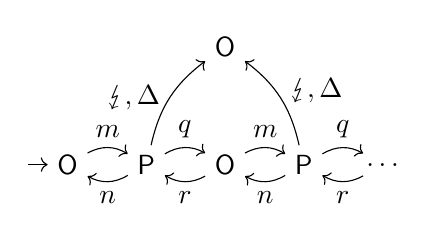
\begin{tikzpicture}[baseline=(O1.base)]
    \node (O1) at (0,0) {\kw{O}};
    \node (P1) at (1,0) {\kw{P}};
    \node (O2) at (2,0) {\kw{O}};
    \node (P2) at (3,0) {\kw{P}};
    \node (O3) at (4,0) {$\ldots$};
    \node (H) at (2,1.5) {\kw{O}};
    \path [->] (-0.5,0) edge (O1);
    \path [->] (O1) edge[bend left] node[auto] {$m$} (P1);
    \path [->] (P1) edge[bend left] node[auto] {$n$} (O1);
    \path [->] (P1) edge[bend left] node[auto] {$q$} (O2);
    \path [->] (P1) edge[bend left=20] node[auto,anchor=east] {$\lightning, \Delta$} (H);
    \path [->] (O2) edge[bend left] node[auto] {$r$} (P1);
    \path [->] (O2) edge[bend left] node[auto] {$m$} (P2);
    \path [->] (P2) edge[bend left] node[auto] {$n$} (O2);
    \path [->] (P2) edge[bend left] node[auto] {$q$} (O3);
    \path [->] (P2) edge[bend right=20] node[anchor=base west] {$\lightning, \Delta$} (H);
    \path [->] (O3) edge[bend left] node[auto] {$r$} (P2);
  \end{tikzpicture}
  \quad
  \begin{array}{c@{\,}lc@{\,}l}
    m &\in M_B^\kw{Q} & q &\in M_A^\kw{Q} \\[1ex]
    n &\in M_B^\kw{A} & r &\in M_A^\kw{A}
  \end{array}
\]
The first move is always a question $m$ played by $\kw{O}$ in $B$.
The player $\kw{P}$ can conclude the current instance of $B$
with an answer $n$, or
initiate an instance of $A$
with a question $q$.
Then $\kw{O}$ can initiate a new instance of $B$
with another $m$, or
conclude any current instance of $A$
with an answer $r$.
This process goes on indefinitely.

To formalize the plays and strategies of $A \rightarrow B$
in a way that accounts for refinement,
we decouple two aspects of this structure.
The following definition of plays
enforces the alternation between $\kw{O}$ and $\kw{P}$.

\begin{definition} % arrow game {{{
Given two elementary games $A$ and $B$,
the moves of the arrow game $A \rightarrow B$
are the questions and answers of $A$ and $B$,
categorized as follows:
\begin{align*}
  M_{A \rightarrow B}^\kw{O} &= M_A^\kw{A} + M_B^\kw{Q} &
  M_{A \rightarrow B}^\kw{Q} &= M_A^\kw{Q} + M_B^\kw{Q} \\
  M_{A \rightarrow B}^\kw{P} &= M_A^\kw{Q} + M_B^\kw{A} &
  M_{A \rightarrow B}^\kw{A} &= M_A^\kw{A} + M_B^\kw{A}
\end{align*}
The \emph{plays} are taken in
the prefix closure $P_{A \rightarrow B}$ of the set:
\[
    (M_{A \rightarrow B}^\kw{O}
     M_{A \rightarrow B}^\kw{P})^* \,
    (\varepsilon +
     M_{A \rightarrow B}^\kw{O} \Delta +
     M_{A \rightarrow B}^\kw{O} \lightning) \,.
\]
Note that
even-length plays represent positions where $\kw{O}$ is expected to play,
whereas odd-length plays represent positions where $\kw{P}$ is.
We write $P_{A \rightarrow B}^\kw{even}$ and $P_{A \rightarrow B}^\kw{odd}$
for the corresponding subsets of $P_{A \rightarrow B}$.
\end{definition}
%}}}

The ``stack discipline'' associating questions
with their eventual answer is captured by
the way we extend refinement conventions to
the plays of $A \rightarrow B$.

\begin{definition} % F_A->B %{{{
Given
$\mathbb{C}_A : \mathcal{R}(A_1, A_2)$ and
$\mathbb{C}_B : \mathcal{R}(B_1, B_2)$,
we can define the following relations
between the moves of $A_1 \rightarrow B_2$
and the moves of $A_2 \rightarrow B_2$:
\begin{align*}
  {\preceq}_{\mathbb{C}_A \rightarrow \mathbb{C}_B}^\kw{O} &=
    {\preceq}_{\mathbb{C}_A}^\kw{A} +
    {\preceq}_{\mathbb{C}_B}^\kw{Q} &
  {\preceq}_{\mathbb{C}_A \rightarrow \mathbb{C}_B}^\kw{Q} &=
    {\preceq}_{\mathbb{C}_A}^\kw{Q} +
    {\preceq}_{\mathbb{C}_B}^\kw{Q} \\
  {\preceq}_{\mathbb{C}_A \rightarrow \mathbb{C}_B}^\kw{P} &=
    {\preceq}_{\mathbb{C}_A}^\kw{Q} +
    {\preceq}_{\mathbb{C}_B}^\kw{A} &
  {\preceq}_{\mathbb{C}_A \rightarrow \mathbb{C}_B}^\kw{A} &=
    {\preceq}_{\mathbb{C}_A}^\kw{A} +
    {\preceq}_{\mathbb{C}_B}^\kw{A} \,,
\end{align*}
The Kripke frame
$\mathcal{F}_{\mathbb{C}_A \rightarrow \mathbb{C}_B} =
 \langle W_{\mathbb{C}_A \rightarrow \mathbb{C}_B}, \leadsto \rangle$
has worlds in
$W_{\mathbb{C}_A \rightarrow \mathbb{C}_B} =
 (W_{\mathbb{C}_A} + W_{\mathbb{C}_B})^*$,
and its accessibility relation $\leadsto$
relates moves of $A_1 \rightarrow B_1$
to moves of $A_2 \rightarrow B_2$,
as defined by the rules:
\[
    \AxiomC{$m_1 \ifr{w \Vdash {\preceq}_{\mathbb{C}_A \rightarrow \mathbb{C}_B}^\kw{Q}} m_2$}
    \UnaryInfC{$\vec{w} \stackrel{m_1, m_2}{\leadsto} w :: \vec{w}$}
    \DisplayProof
    \quad
    %\begin{array}{c}
    %  \vec{w} \stackrel{\#,\#}{\leadsto} \vec{w} \\[0.7ex]
    %  \vec{w} \stackrel{\tau, \tau}{\leadsto} \vec{w}
    %\end{array}
    %\quad
    \AxiomC{$m_1 \ifr{w \Vdash {\preceq}^\kw{A}_{\mathbb{C}_A \rightarrow \mathbb{C}_B}} m_2$}
    \UnaryInfC{$w :: \vec{w} \stackrel{m_1, m_2}{\leadsto} \vec{w} \,.$}
    \DisplayProof
\]
%Then two plays are related at $\vec{w}$
%when there is a path from $\varepsilon$ to $\vec{w}$
%in $\leadsto$ whose labels project onto the plays:
%\[
%    \AxiomC{$s : \varepsilon \leadsto^* \vec{w}$}
%    \UnaryInfC{$\pi_1^*(s)
%       \ifr{\vec{w} \Vdash {\preceq}_{A \rightarrow B}}
%       \pi_2^*(s)$}
%    \DisplayProof
%\]
%If
%$\langle A, \mathbb{C}_A \rangle$ and
%$\langle B, \mathbb{C}_B \rangle$
%are two games with refinement, then
%a \emph{valid play} of $A \rightarrow B$
%is a sequence $s \in P_{A \rightarrow B}$
%such that $(s, s) \in [\vec{w} \Vdash {\preceq}_{A \rightarrow B}]$
%for some $\vec{w}$.
\end{definition}

The frame $\mathcal{F}_{\mathbb{C}_A \rightarrow \mathbb{C}_B}$
is used in \S\ref{sec:sim}
to define our notion of simulation.
%}}}

%}}}

%}}}

\subsection{Behavior specifications} %{{{

By contrast with more traditional settings,
in our model strategies represent a range of possible behaviors
of the system and as such are not expected to be deterministic.
In addition,
our explicit treatment of divergence,
the possibility for strategies to exhibit undefined behaviors,
and our commitment to strategy refinement as a first-class citizen
[...]

In this section,
we capture these aspects of our model
in the \emph{behavior specification} monad.

\subsubsection{Definition}

Given a base type $A$,
a computation in $A$ may produce 
may produce a value of type $A$,
but it may also diverge or exhibit undefined behavior.
Hence,
a behavior specification for $A$ is an element:
\[
    x \in \mathcal{B}(A) = \mathcal{P}(A + \{ \Delta, \lightning \})
\]
The unit of $\kw{ret}_A : A \rightarrow \mathcal{B}(A)$
of the monad $\mathcal{B}$ is given by:
\[
    \kw{ret}_A(a) = \{ a \} \,,
\]
and the binding operation is defined in the following way:
\[
    \AxiomC{$a \in x$}
    \AxiomC{$b \in f(a)$}
    \BinaryInfC{$b \in x >>= f$}
    \DisplayProof
    \quad
    \AxiomC{$\Delta \in x$}
    \UnaryInfC{$\Delta \in x >>= f$}
    \DisplayProof
    \quad
    \AxiomC{$\lightning \in x$}
    \UnaryInfC{$\lightning \in x >>= f$}
    \DisplayProof
\]
The usual monad laws hold, and
the Kleisi composition of $f : A \rightarrow \mathcal{B}(B)$ and
$g : B \rightarrow \mathcal{B}(C)$ can be derived as:
\[
    (f \cdot g)(a) = (f(a) >>= g) \,.
\]
The action of $\mathcal{B}$ on functions can be derived as:
\[
    \mathcal{B}(f) = x \mapsto (x >>= \kw{ret}_A \circ f) \,.
\]


\subsubsection{Refinement}

We can promote a relation $R : \mathcal{R}(A, B)$
to behavior specifications as:
\[ \mathcal{B}^+(R) :=
   \mathcal{P}^+(R + \{ (\Delta, \Delta), (x, \lightning) \mid x \in A \}) \]
Note that $\mathcal{B}$ preserves reflexivity and transitivity,
so that if $\sqsubseteq$ is a preorder,
then $\mathcal{B}(\sqsubseteq)$ is a preorder as well.

The least and greatest elements
can be defined as:
\[ \bot := \varnothing \qquad \top := \{ \lightning \} \,, \]
with the property that for all $R, x, S$:
\[ \bot \ifr{\mathcal{B}^+(R)} x \ifr{\mathcal{B}^+(S)} \top \,. \]

In addition,
for $R : \mathcal{R}(A_1, A_2)$ and $S : \mathcal{R}(B_1, B_2)$,
the monad operations satisfy the expected relational properties:
\begin{gather*}
\kw{ret}_{A_1} \ifr{R \rightarrow \mathcal{B}^+(R)} \kw{ret}_{A_2} \\
({>>=}) \ifr{\mathcal{B}^+(R) \rightarrow (R \rightarrow \mathcal{B}^+(S))
  \rightarrow \mathcal{B}^+(S)} ({>>=}) \\
{\cdot} \ifr{(R \rightarrow \mathcal{B}^+(S)) \rightarrow
             (S \rightarrow \mathcal{B}^+(T)) \rightarrow
             (R \rightarrow \mathcal{B}^+(T))} {\cdot} \\
\mathcal{B}(-) \ifr{(R \rightarrow S) \rightarrow (\mathcal{B}^+(R)
\rightarrow \mathcal{B}^+(S))} \mathcal{B}(-)
\end{gather*}

\subsubsection{Kleene star}

A Kleisli morphism of type $f : A \rightarrow \mathcal{B}(A)$
can be interpreted as a transition relation on the set of states $A$,
and we can define the iteration $f^*$
in a way that recognizes silent divergence.
Writing $f^n$ for the $n$-fold composition of the form
$f \cdot f \cdots f$,
divergence can be recognized as:
\[ \kw{diverges}_f(a) \Leftrightarrow
    \forall n \in \mathbb{N} \,.\,
    \exists a' \in A \,.\,
    f^n(a) \ni a' \]
Nondeterministic choice
and its unit can be defined as:
\[ f + g := a \mapsto f(a) \cup g(a)  \qquad  0 := a \mapsto \bot \]
Then the iteration of $f$ is:
\[ f^* := \sum_{n \in \mathbb{N}} f^n +
          (a \mapsto \{ \Delta \mid \kw{diverges_f(a)} \}) \]

Using Kleisi composition as multiplication,
the structure
$\langle A \rightarrow \mathcal{B}(A), {\cdot}, {+}, \kw{ret}_A, 0, * \rangle$
is analogous to a Kleene algebra.
However, as noted in \cite{failkat},
the possibility of an abnormal outcome
means that annihilation of $\cdot$ by $0$ on the right
does not hold.
In particular:
\[ \Delta \cdot 0 = \Delta \qquad \lightning \cdot 0 = \lightning \]

Nevertheless,
this notion of iteration
and the associated equational theory
will be useful
for defining strategies operationally,
in terms of small-step transition relations.

%}}}

\subsection{Strategies} %{{{

A strategy for $A \rightarrow B$
is essentially a tree
which gathers the possible interactions of
the system being modeled.
We give a traditional representation
as a prefix-closed set of plays,
but will work with strategies defined as transition systems.

\subsubsection{Traces} %{{{

In the existing literature,
strategies are usually formalized as prefix-closed sets of plays.
This establishes a connection with trace semantics of process calculi.
In our case,
a strategy given in this form is a set:
\[ \sigma \subseteq P_{A \rightarrow B} \,, \]
which satisfies
for all $st \in P_{A \rightarrow B}$
and $m \in M_{A \rightarrow B}^\kw{O}$:
\begin{itemize}
  \item $st \in \sigma \Rightarrow s \in \sigma$;
  \item $s \in \sigma \wedge sm \in P_{A \rightarrow B}
    \Rightarrow sm \in \sigma$.
\end{itemize}
The first condition ensures that $\sigma$ is prefix-closed,
whereas the second condition ensures that
all possible behaviors of $\kw{O}$ are included
at all reachable positions.

XXX require downward closure wrt $\lightning$
so that unique and ordered by inclusion.

%}}}

\subsubsection{Transition systems} %{{{

Instead of manipulating sets of traces directly,
we will define strategies using a specialized form of transition system.

\begin{definition} % strategy {{{
\label{def:strat}
An \emph{strategy} $\sigma$ for the arrow game $A \rightarrow B$
is a tuple
$\langle K, S,
{\xrightarrow{\kw{O}} },
{\xrightarrow{\tau}},
{\xrightarrow{\kw{P}} },
 \#, k_0 \rangle$
where:
\begin{itemize}
  \item $K$ is a set of \emph{continuation states};
  \item $S$ is a set of \emph{running states};
  \item ${\stackrel{\kw{O}}{\rightarrow}} :
         K \rightarrow
         M_{A \rightarrow B}^\kw{O} \rightarrow
         \mathcal{P}(S^\lightning)$
    is a \emph{resumption relation};
  \item ${\stackrel{\tau}{\rightarrow}} :
         S \rightarrow \mathcal{P}(S^\lightning)$
    is an \emph{internal transition relation};
  \item ${\stackrel{\kw{P}}{\rightarrow}} :
         S \rightarrow \mathcal{P}(M_{A \rightarrow B}^\kw{P} \times K)$
    is a \emph{suspension relation};
  \item ${\#} : K \rightarrow \mathcal{P}(M_B^\kw{Q})$
    is a \emph{refusal relation};
  \item $k_0$
    is the strategy's \emph{initial continuation}.
\end{itemize}
The set of states is extended to $S^\lightning = S \uplus \{\lightning\}$
so that $\sigma$ may perform a transition to $\lightning$
whenever an undefined behavior is encountered.
We will write:
\begin{itemize}
  \item $k \xrightarrow{m} s$ when ${\xrightarrow{\kw{O}} }(k, m) \ni s$, and
  \item $s \xrightarrow{m} k$ when ${\xrightarrow{\kw{P}} }(s) \ni (m, k)$.
\end{itemize}
We write $\sigma : A \rightarrow B$ when $\sigma$ is a strategy
for $A \rightarrow B$.
\end{definition}
%}}}

Continuations correspond to
the points in the execution where $\kw{O}$ is expected to move,
whereas states correspond to
the points where $\kw{P}$ is expected to move.
The set of traces associated with a state is
defined by mutual recursion as:
\[
  \begin{array}{l@{\:}c@{\:\{}l@{\:\mid\:}l}
    \kw{traces}_\sigma(k) & = & \varepsilon, m &
      m \in M_{A \rightarrow B}^\kw{O} \} \\
    & \cup & m t &
      k \xrightarrow{m} s \wedge t \in \kw{traces}_\sigma(s) \} \\
    & \cup & m \# &
      k \: \# \: m \} \\
    \kw{traces}_\sigma(s) & = & \tau, \tau t &
      s \xrightarrow{\tau} s' \wedge t \in \kw{traces}_\sigma(s') \} \\
    & \cup & m t &
      s \xrightarrow{m} k \wedge t \in \kw{traces}_\sigma(k) \} \\
    & \cup & \lightning & s = \lightning \}
  \end{array}
\]
Then the behavior of strategies can be made explicit
by specifying the corresponding sets of plays as:
\[
  \kw{traces}(\sigma) = \kw{traces}_\sigma(k_0) \,.
\]

XXX downward closure wrt $\lightning$

[Show that $\subseteq P_{A \rightarrow B}$,
and that it satisfies the requirements outlined
in the previous section.]

[Advantages: alternation structure baked in,
can be handled by the proof assistant's type system.
Facilitates embedding of operational semantics,
and intuitive operational reasoning.]

[Inconvenient: junk and non unique,
but we don't care because we're going to
define simulations and quotient anyway.]

%}}}

%}}}

\subsection{Simulations} %{{{
\label{sec:sim}

Having formally defined a notion of strategy
for the game $A \rightarrow B$,
we turn to the corresponding relational notion of simulation
for the refinement convention $\mathbb{C}_A \rightarrow \mathbb{C}_B$.
To this end,
we first introduce the following modal constructions.

\begin{definition} % modal relators for simulation {{{
For frames labelled by pairs
($\Lambda = \Lambda_1 \times \Lambda_2$),
we define variants of $\Box, \Diamond$ which
allow world transitions to interact with the components
being related.
The relators:
\begin{align*}
  \Diamond \times {-} &: \mathcal{R}_W(A, B) \rightarrow
              \mathcal{R}_W(\Lambda_1 \times A, \, \Lambda_2 \times B) \\
  \Box \rightarrow - &: \mathcal{R}_W(A, B) \rightarrow
          \mathcal{R}_W(\Lambda_1 \rightarrow A, \, \Lambda_2 \rightarrow B) \\
  \mathcal{P}^+(\Box) &:
      \mathcal{R}_W(\mathcal{P}(\Lambda_1), \mathcal{P}(\Lambda_2))
\end{align*}
are defined as:
\begin{gather*}
  (l_1, a) \ifr{w \Vdash \Diamond \times R} (l_2, b) \Leftrightarrow
    a \ifr{w \Vdash \langle l_1, l_2 \rangle R} b \\
  f \ifr{w \Vdash \Box \rightarrow R} g \Leftrightarrow
    \forall \, l_1 l_2 \,.\, f(l_1) \ifr{w \Vdash [l_1, l_2] R} g(l_2) \\
  L_1 \ifr{w \Vdash \mathcal{P}^+(\Box)} L_2 \Leftrightarrow
    \forall \, w \stackrel{l_1, l_2}{\leadsto} w' \,.\,
      l_1 \in L_1 \Rightarrow l_2 \in L_2 \,.
\end{gather*}
\end{definition}
%}}}

With these constructions,
our notion of simulation relation
is naturally derived from
the types we used to define strategies (Def.~\ref{def:strat}).
They are used
with respect to the frame $\mathcal{F}_{A \rightarrow B}$
defined in \S\ref{sec:arrow}.
Hence, the simulation operates in the context of
a stack of elementary worlds
specifying how answers to pending questions
should be related.
In each one of the component games $A_i$ and $B_i$,
answers will be related at the same world as the corresponding questions:
$\kw{P}$ can rely on $\kw{O}$ making this true for $A$;
it must guarantee that this is true for $B$.

\begin{definition} % simulation relation {{{
Given
$\mathbb{C}_A : \mathcal{R}(A_1, A_2)$,
$\mathbb{C}_B : \mathcal{R}(B_1, B_2)$
two refinement conventions, and
$\sigma_1 : A_1 \rightarrow B_1$,
$\sigma_2 : A_2 \rightarrow B_2$
two strategies,
a \emph{simulation relation} between $\sigma_1$ and $\sigma_2$
is a pair of relations $R = \langle R_S, R_K \rangle$ with
$R_K : \mathcal{R}_{W_{\!A \rightarrow B}}(K_1, K_2)$ and
$R_S : \mathcal{R}_{W_{\!A \rightarrow B}}(S_1, S_2)$
such that:
\begin{gather*}
  \xrightarrow{\kw{O}}_1
  \ifr{\Vdash R_K \rightarrow \Box \rightarrow \mathcal{P}^+(R_S^\lightning)}
  \xrightarrow{\kw{O}}_2
  \\
  \xrightarrow{\tau}_1
  \ifr{\Vdash R_S \rightarrow \mathcal{P}^+(R_S^\lightning)}
  \xrightarrow{\tau}_2
  \\
  \xrightarrow{\kw{P}}_1
  \ifr{\Vdash R_S \rightarrow \mathcal{P}^+(\Diamond \times R_K)}
  \xrightarrow{\kw{P}}_2
  \\
  \#_1
  \ifr{\Vdash R_K \rightarrow \Box \rightarrow {\Rightarrow}}
  \#_2
  \\
  k_{0,1} \ifr{\varepsilon \Vdash R_K} k_{0,2}
\end{gather*}
The relation on states is extended to:
\[
    R_S^\lightning =
    R_S \cup \{ (s_1, \lightning) \mid s_1 \in S_1^\lightning \} \,.
\]
We will write
$\sigma_1 \le_{\mathbb{C}_A \rightarrow \mathbb{C}_B}^R \sigma_2$
when $R$ is a simulation relation in this sense, and write
$\sigma_1 \le_{\mathbb{C}_A \rightarrow \mathbb{C}_B} \sigma_2$
when there exists any such simulation relation.
\end{definition}
%}}}

%}}}

\subsection{Operators} %{{{

\subsubsection{Multi-component games and strategies} %{{{

The simplest way to aggregate a family of strategies $(\sigma_i)_{i\in I}$
is to annotate all of the moves exchanged by the system with its environment
by a component identifier $i$.

\begin{definition} % multi-channel game {{{
For an elementary game $A$ and a set $I$,
we define the \emph{multi-channel game}
$A^I = \langle I \times M_G^\kw{Q}, I \times M_G^\kw{A} \rangle$.
Given a refinement convention
$\mathbb{C} : \mathcal{R}(A_1, A_2)$,
we define
$\mathbb{C}^I =
 \langle W, {\preceq}^\kw{Q}, {\preceq}^\kw{A} \rangle :
 \mathcal{R}(A_1^I, A_2^I)$
where
$W = I \times W_\mathbb{C}$ and
$\preceq^\kw{Q}, \preceq^\kw{A}$
are given by the rules:
\[
    \small
    \AxiomC{$m_1 \ifr{w \Vdash {\preceq}_\mathbb{C}^\kw{Q}} m_2$}
    \UnaryInfC{$(i, m_1) \ifr{(i, w) \Vdash {\preceq}^\kw{Q}} (i, m_2)$}
    \DisplayProof
    \quad
    \AxiomC{$m_1 \ifr{w \Vdash {\preceq}_\mathbb{C}^\kw{A}} m_2$}
    \UnaryInfC{$(i, m_1) \ifr{(i, w) \Vdash {\preceq}^\kw{A}} (i, m_2)$}
    \DisplayProof
\]
\end{definition}
%}}}

The aggregated strategy uses the labels to direct each move
to the corresponding component,
and lets the components operate independently.

\begin{definition} % multi-component strategy {{{
For a family of strategies
$\vec{\sigma} = (\sigma_i)_{i \in I}$
with
$\sigma_i = \langle K_i, S_i, \xrightarrow{\kw{O}}_i,
  \xrightarrow{\tau}_i, \xrightarrow{\kw{P}}_i, \#_i, k_{0i} \rangle :
  A \rightarrow B$,
the multi-component strategy
$\mathcal{M}(\sigma_i)_{i \in I} : A^I \rightarrow B^I$
is defined over the sets of states:
\[
  K := \prod_{i \in I} K_i \qquad
  S := \sum_{i \in I}
    \Big( S_i \times \prod_{i \ne j} K_j \Big)
\]
by the following rules:
\[
  \begin{array}{c@{\qquad}c}
    \AxiomC{$k_i \xrightarrow{m}_i s$}
    \UnaryInfC{$\vec{k} \xrightarrow{(i, m)} (i, s, \vec{k} \backslash i)$}
    \DisplayProof
    &
    \AxiomC{$s \xrightarrow{m}_i k_i$}
    \UnaryInfC{$(i, s, \vec{k} \backslash i) \xrightarrow{(i, m)} \vec{k}$}
    \DisplayProof
    \\[1.5em]
    \AxiomC{$s \xrightarrow{\tau}_i s'$}
    \UnaryInfC{$(i, s, \vec{k}) \xrightarrow{\tau} (i, s', \vec{k})$}
    \DisplayProof
    &
    \AxiomC{$k \: \#_i \: m$}
    \UnaryInfC{$\vec{k} \: \# \: (i, m)$}
    \DisplayProof
  \end{array}
\]
and uses the initial continuation $(k_{0i})_{i \in I}$.
\end{definition}
%}}}

In other words,
at most one component is active at any time,
and the others remain in continuation states.
A resumption activates the component whose index
is read from the move,
and the index is incoroporated back into
any move played by the component.

\begin{lemma} % monotonicity {{{
For a family of simulation relations $\vec{R} = (R_i)_{i \in I}$ such that
$\sigma_{1,i} \le_{\mathbb{C}_A \rightarrow \mathbb{C}_B}^{R_i} \sigma_{2,i}$,
the relation $\mathcal{M}(\vec{R})$ defined by:
\begin{gather*}
  \AxiomC{$\forall i \,.\,
    k_{1,i} \ifr{\vec{w} \restriction i \Vdash R_{K,i}} k_{2,i}$}
  \UnaryInfC{$\vec{k_1} \ifr{\vec{w} \Vdash \mathcal{M}(\vec{R})_K} \vec{k_2}$}
  \DisplayProof
  \\[.5ex]
  \AxiomC{$s_1 \ifr{\vec{w} \restriction i \Vdash R_{S,i}} s_2$}
  \AxiomC{$\forall j \ne i \,.\,
    k_{1,j} \ifr{\vec{w} \restriction j \Vdash R_{S,j}} k_{2,j}$}
  \BinaryInfC{$(i, s_1, \vec{k}_1)
    \ifr{\vec{w} \Vdash \mathcal{M}(\vec{R})_S}
    (i, s_2, \vec{k}_2)$}
  \DisplayProof
\end{gather*}
is a simulation relation between the strategies:
\[
  \mathcal{M}(\vec{\sigma_1})
  \le_{\mathbb{C}_A^I \rightarrow \mathbb{C}_B^I}^{\mathcal{M}(\vec{R})}
  \mathcal{M}(\vec{\sigma_2}) \, .
\]
The stack of worlds $\vec{w} \restriction i$
is the sequence $w_1, w_2, \ldots, w_n$
such that $(i, w_1), (i, w_2), \ldots, (i, w_n)$
is the subsequence of $\vec{w}$ containing worlds
paired with $i$ indices.
\end{lemma}
%}}}

%}}}

\subsubsection{Flat composition} %{{{

Once we have such an aggregate,
we can ``flatten'' the communication between
the system and the environment
back to the unannotated game $A \rightarrow B$.

\begin{definition} % flattening {{{
The \emph{flattening} of $\sigma : A^I \rightarrow B^I$
is the strategy $\sigma^\rhd : A \rightarrow B$
defined over the sets of states
$K := K_\sigma \times I^*$ and
$S := S_\sigma \times I^*$ by the following rules:
\[
  \begin{array}{c@{\quad}c}
    \AxiomC{$k \xrightarrow{(i, m)}_\sigma s$}
    \AxiomC{$\forall \, j \ne i \,.\, k \: \#_{\!\sigma} \: (j, m)$}
    \BinaryInfC{$(k, \iota) \xrightarrow{m} (s, \iota)$}
    \DisplayProof
    &
    \AxiomC{$s \xrightarrow{(i, n)}_\sigma k$}
    \UnaryInfC{$(s, \iota) \xrightarrow{n} (k, \iota)$}
    \DisplayProof
    \\[1.5em]
    \AxiomC{$s \xrightarrow{(i, q)}_\sigma k$}
    \UnaryInfC{$(s, \iota) \xrightarrow{q} (k, i :: \iota)$}
    \DisplayProof
    &
    \AxiomC{$k \xrightarrow{(i, r)}_\sigma s$}
    \UnaryInfC{$(k, i :: \iota) \xrightarrow{r} (s, \iota)$}
    \DisplayProof
    \\[1.5em]
    \AxiomC{$s \xrightarrow{\tau}_\sigma s'$}
    \UnaryInfC{$(s, \iota) \xrightarrow{\tau} (s', \iota)$}
    \DisplayProof
    &
    \AxiomC{$\forall \,i\,.\, k \: \#_{\!\sigma} \: (i, m)$}
    \UnaryInfC{$(k, \iota) \:\#\: m$}
    \DisplayProof
  \end{array}
\]
\end{definition}
%}}}

We direct an incoming question in $B$
to a component $i$ when all other components reject it.
If the component then asks a question in the game $A$,
we save its identifier on the stack $\iota$,
so that the corresponding answer can be directed back to $i$.

\begin{lemma}
Given a simulation relation
$\sigma_1 \le_{\mathbb{C}_A^I \rightarrow \mathbb{C}_B^I}^R \sigma_2$,
the relation $R^\rhd$ is defined for continuation states by:
\[
  \AxiomC{$k_1 \ifr{\vec{w} \Vdash R_K} k_2$}
  \AxiomC{$\iota = \pi_1^*(\vec{w}) \mbox{ XXX}$}
  \BinaryInfC{
    $(k_1, \iota) \ifr{\pi_2^*(\vec{w}) \Vdash R^\rhd_K} (k_2, \iota)$}
  \DisplayProof
\]
and similarly for running states.
$R^\rhd$ is a simulation relation:
\[
    \sigma_1^\rhd
    \le_{\mathbb{C}_A \rightarrow \mathbb{C}_B}^{R^\rhd}
    \sigma_2^\rhd \,.
\]
\end{lemma}

Putting together multi-component strategies and flattening,
the \emph{flat composition} operator
$\mathcal{F} : [A \rightarrow B] \rightarrow [A \rightarrow B]$
is:
\[
    \mathcal{F}(\vec{\sigma}) := \mathcal{M}(\vec{\sigma})^\rhd
\]
This allows us to bundle multiple components of the same type,
however note that so far they do not interact with each other
(only to decide who's going to handle what question).

%}}}

\subsubsection{Resolution operator} %{{{

To allow interaction within a composite system,
we define the following resolution operator,
which feeds back a strategy's own questions to itself
whenever possible.

\begin{definition} % resolution {{{
The \emph{resolution} of $\sigma : A \rightarrow A$,
written $\mathcal{R}(\sigma)$,
is defined over the sets of states
$K := K_\sigma \times \{\kw{O}, \kw{P}\}^*$ and
$S := S_\sigma \times \{\kw{O}, \kw{P}\}^*$
by the following rules:
\[
  \begin{array}{cc}
    {\small m \in M_A^\kw{Q}, \:\: n \in M_A^\kw{A}}
    &
    {\small q \in M_A^\kw{Q}, \:\: r \in M_A^\kw{A}}
    \\[1em]
    \AxiomC{$k \xrightarrow{m}_\sigma s$}
    \UnaryInfC{$(k, \iota) \xrightarrow{m} (s, \kw{O} :: \iota)$}
    \DisplayProof
    &
    \AxiomC{$s \xrightarrow{n}_\sigma k$}
    \UnaryInfC{$(s, \kw{O} :: \iota) \xrightarrow{n} (k, \iota)$}
    \DisplayProof
    \\[1.5em]
    \AxiomC{$s \xrightarrow{q}_\sigma k$}
    \AxiomC{$k \:\#_{\!\sigma}\: q$}
    \BinaryInfC{$(s, \iota) \xrightarrow{q} (k, \iota)$}
    \DisplayProof
    &
    \AxiomC{$k \xrightarrow{r}_\sigma s$}
    \UnaryInfC{$(k, \iota) \xrightarrow{r} (s, \iota)$}
    \DisplayProof
    \\[1.5em]
    \AxiomC{$s \xrightarrow{q}_\sigma k$}
    \AxiomC{$k \xrightarrow{q}_\sigma s'$}
    \BinaryInfC{$(s, \iota) \xrightarrow{\tau} (s', \kw{P} :: \iota)$}
    \DisplayProof
    &
    \AxiomC{$s \xrightarrow{r}_\sigma k$}
    \AxiomC{$k \xrightarrow{r}_\sigma s'$}
    \BinaryInfC{$(s, \kw{P} :: \iota) \xrightarrow{\tau} (s', \iota)$}
    \DisplayProof
    \\[1.5em]
    \AxiomC{$s \xrightarrow{\tau}_\sigma s'$}
    \UnaryInfC{$(s, \iota) \xrightarrow{\tau} (s', \iota)$}
    \DisplayProof
    &
    \AxiomC{$k \:\#_{\!\sigma}\: m$}
    \UnaryInfC{$(k, \iota) \:\#\: m$}
    \DisplayProof
  \end{array}
\]
The initial continuation is $(k_{\sigma}, \varepsilon)$.
\end{definition}
%}}}

\begin{lemma}
If
$\sigma_1 \le_{\mathbb{C}_A \rightarrow \mathbb{C}_A}^R \sigma_2$,
then
$\mathcal{R}(\sigma_1)
 \le_{\mathbb{C}_A \rightarrow \mathbb{C}_A}^{\mathcal{R}(R)}
 \mathcal{R}(\sigma_2)$,
where $\mathcal{R}(R)$ is defined as follows.
For a world $\vec{w} \in W_{A \rightarrow B}$
and a stack $\iota \in \{\kw{O}, \kw{P}\}^*$,
the set $\mathcal{R}_\iota(\vec{w}) \subseteq W_{A \rightarrow B}$
is defined by the following rules together with the base case
$\varepsilon \in \mathcal{R}_\varepsilon(\varepsilon)$:
\[
    \AxiomC{$\vec{w}' \in \mathcal{R}_\iota(\vec{w})$}
    \UnaryInfC{$x :: \vec{w}' \in \mathcal{R}_{\kw{O} :: \iota}(x :: \vec{w})$}
    \DisplayProof
    \quad
    \AxiomC{$\vec{w}' \in \mathcal{R}_\iota(\vec{w})$}
    \UnaryInfC{$x :: x :: \vec{w}' \in \mathcal{R}_{\kw{P} :: \iota}(\vec{w})$}
    \DisplayProof
\]
XXX this is only the rules for codomain worlds,
we need a case for domain worlds to be passed along.

Then the relation $\mathcal{R}(R)$ is given for continuation states by:
\[
  \AxiomC{$k_1 \ifr{\vec{w} \Vdash R_K} k_2$}
  \AxiomC{$\vec{w}' \in \mathcal{R}_\iota(\vec{w})$}
  \BinaryInfC{$(k_1, \iota) \ifr{\vec{w}' \Vdash \mathcal{R}(R)_K} (k_2, \iota)$}
  \DisplayProof
\]
and similarly for running states.

XXX the proof needs $\mathcal{R}(\vec{w})$ to take into account
whether the component is currently running (states) or not (continuations).
\end{lemma}

%}}}

\subsubsection{Observation operator} %{{{

The simulations defined in \S\ref{sec:sim}
only relate strategies whose internal actions match one-to-one.
However, the operator defined in this section
will allow us to normalize strategies by removing
all finite sequences of $\tau$s.

\begin{definition}
Given $\sigma : A \rightarrow B$,
the \emph{observation strategy}
$\sigma \backslash \tau^* =
 \langle K_\sigma, S_\sigma \uplus \{\ast\},
         \xrightarrow{\kw{O}},
         \xrightarrow{\tau},
         \xrightarrow{\kw{P}}_\sigma,
         \#_\sigma, k_{0,\sigma} \rangle$
uses the resumption and internal transition relations
defined by the rules:
\[
  \AxiomC{$s \xrightarrow{\tau}_\sigma s'$}
  \AxiomC{$s' \xrightarrow{\tau^\omega}$}
  \doubleLine \BinaryInfC{$s \xrightarrow{\tau^\omega}$}
  \DisplayProof
  \qquad
  \AxiomC{$k \xrightarrow{m}_\sigma s$}
  \AxiomC{$s \xrightarrow{\tau^\omega}$}
  \BinaryInfC{$k \xrightarrow{m} \ast$}
  \DisplayProof
\]\[
  \AxiomC{$k \xrightarrow{m}_\sigma s$}
  \AxiomC{$s \xrightarrow{\tau^*}_\sigma s' \xrightarrow{n}_\sigma k'$}
  \BinaryInfC{$k \xrightarrow{m} s'$}
  \DisplayProof
  \qquad
  \ast \xrightarrow{\tau} \ast \,.
\]
\end{definition}

\begin{lemma}
If $\sigma_1 \le_{\mathbb{C}_A \rightarrow \mathbb{C}_B}^R \sigma_2$,
then for $R \backslash \tau^* = R \cup \{(\ast, \ast)\}$
the following holds:
\[
  \sigma_1 \backslash \tau^*
  \le_{\mathbb{C}_A \rightarrow \mathbb{C}_B}^{R \backslash \tau^*}
  \sigma_2 \backslash \tau^* \,.
\]
\end{lemma}

%}}}

%}}}

{ \color{gray}
Note that for both states and continuations,
nondeterminism is interpreted as \emph{output} nondeterminism,
as prescribed by the use of the relator $\mathcal{P}^+$.
This means that alternating transition system
implicitely accept all possible inputs from the environment,
although some of them may cause the system to immediately go wrong.
Likewise,
the special resumption $\kw{refuse}$
is taken as a positive, output behavior from the system,
rather than a restriction on the environment ---
this will be important to establish the monotonicity
of the composition operator defined in Sec.~\ref{?}.
This approach corresponds to the saturation requirement on strategies
often found in traditional game semantics,
or notions of receptiveness used in CompCert
and in concurrency theory.

Furthermore, we need to distinguish between mere nondeterminism
and \emph{branching}.
This is explored in the following section.

\subsection{Branching and determinism}

Whereas nondeterminism allows a strategy to posess
multiple observable behaviors,
branching occurs when multiple state transitions
are associated with the same immediate observable behavior.
This can create spurious distinctions,
whereby systems that yield the same sets of traces
cannot be identified by simulation,
and as such we consider it undesirable.
The following definition
formalizes the conditions a transition system must satisfy
to be considered free from branching.

\begin{definition}[Nonbranching transition system]
For given sets of moves and states,
a continuation $k : M \rightarrow \mathcal{P}(\kw{resumption}(S))$
is \emph{nonbranching} if the following property holds:
\[ \forall m \,.\, | k(m) | \le 1 \]
A transition system $\alpha : \kw{ats}(M, S)$ is nonbranching
if the following property holds:
\[ \forall s, m, k_1, k_2 \,.\,
     \alpha(s) \supseteq \{ m \cdot k_1, m \cdot k_2 \} \Rightarrow
     k_1 = k_2 \,, \]
and if for all $s, m, k$ such that $\alpha(s) \ni \underline{m} \cdot k$,
the continuation $k$ is nonbranching.
\end{definition}

Determinism is a stronger property,
and ensures that the system has at most one possible behavior
at any point.
We expect the semantics of concrete systems ---
as opposed to specifications ---
to be deterministic in the following sense.

\begin{definition}[Deterministic transition system]
For given sets of moves and states,
a transition system $\alpha : \kw{ats}(M, S)$
is deterministic if for all $s$, $|\alpha(s)| \le 1$,
and if for all $s, m, k$ such that $\alpha(s) \ni \underline{m} \cdot k$,
the continuation $k$ is nonbranching.
\end{definition}

Note that both nonbranching and determinism
only relate to the behavior of the system.
In both cases,
the environment remains free to play any move.
Abramsky notes in \cite{cspgs}
that [it's one of the good things about game semantics].

\subsection{Internal actions and divergence}

The emergence of silent divergence
is one of the major difficulties
associated with modeling interacting systems.
Indeed,
two systems which, taken in isolation,
only exhibit reactive behavior,
can nonetheless become silently divergent when composed together,
if it is possible to interact with each other continuously
without intervening communication with the outside.

An operational description of this phenomenon
models this internal interaction explicitly
in the form of silent actions $\tau$.
When comparing the behavior of two systems,
finite sequences of $\tau$'s will be considered equivalent.
However,
silent divergence in the form of an infinite sequence of $\tau$'s
can only correspond to another infinite sequence.
This is usually addressed by the introduction of
sophisticated notions of simulation,
such as the \emph{measure simulations} used for instance in CompCert.

On the other hand,
in most work on denotational semantics,
including traditional game semantics such as \cite{pcfgs},
[complicated fixpoints] 

Our model includes a notion of internal action $\tau$,
which makes it possible to handle silent divergence explicitely
rather than through sophisticated domain-theoretic constructions.
However,
note that the notion of simulation we have defined
does not allow any variation
in the number of internal transitions
between the two transition systems being related.
Nevertheless,
composition operators remain monotonic
under this definition of simulation,
because [...]
Normalize using the following operator.

\begin{definition}[Observation operator]
For a transition system $\alpha : \kw{ats}(M, S)$,
we define the \emph{observations} transition system
$\mathcal{O}(\alpha)$ as follows.
A behavior $r : \kw{behavior}(M, S)$ is said to be
\emph{observable} if $r \ne \tau \cdot s$ for all $s \in S$.
A state $s' \in S$ is said to be \emph{reachable} from $s \in S$
if there is a sequence $s_0, s_1, \ldots s_n$ such that
$s_0 = s$, $s_n = s'$,
and for all $0 \le i < n$
there is a transition $\alpha(s_i) \ni \tau \cdot s_{i+1}$.
A state $s$ is said to be \emph{silently divergent}
if there is an infinite sequence $s_0, s_1, \ldots$
such that $s_0 = s$ and for all $i$,
there is a transition $\alpha(s_i) \ni \tau \cdot s_{i+1}$.
Then the observations transition system is defined as:
\begin{align*}
    \mathcal{O}(\alpha)(s) = &\{ r \:|\: r \mbox{ is observable } \wedge
         \exists s' \,.\, s \rightarrow^* s' \wedge
		\alpha(s') \ni r \} \\
      \cup &\{ \Delta \:|\: s \mbox{ is silently divergent} \}
\end{align*}
\end{definition}

Properties:
preserve nonbranching (if that's defined in the right way), determinism.
Monotonic.

}

\section{Open Modules for Compcert}

Having laid out our basic game framework,
we show how this framework can be used
to construct a compositional semantics for CompCert.

\subsection{Overview}

CompCert is a C-to-assembly compiler written and verified
in the Coq proof assistant.
The compiler is accompanied by
a formal semantics of the source, target, and intermediate languages,
and a proof that if the compiler succeeds,
then the behavior of the emitted target program
refines that of the source program.

The original CompCert
only formalizes the execution of a complete program's
\texttt{int main()} function called with no arguments.
Language semantics interpret external calls
using a predefined behavior for external functions,
common to all languages.
In turn,
the behavior of external functions
defines event traces
recording their interaction with the environment
from of a fixed set of possible actions,
such as volatile memory accesses or the invocation of system calls.
However,
two-way interaction between program modules
cannot be modeled using this facility.

Following Compositional CompCert \cite{compcompcert},
we replace this model by extending the semantics of CompCert programs
in two ways:
\begin{itemize}
\item First,
  we allow the initial and final states of CompCert modules
  to account for a variety of entry points and final configurations,
  so that every function in a program module
  may be invoked with any combination of arguements,
  and so that functions may pass back an arbitrary return value
  and an updated memory state to the caller
  once they terminate;
\item Second,
  rather than computing the semantics of external calls
  using a predefined global parameter,
  our model allows languages semantics to perform external calls explicitely,
  using the same interface they implement for incoming calls.
\end{itemize}
Furthermore,
our model is parametrized by elementary games
specifying the form of the incoming and external calls
used by a given language semantics.
The model is defined formally in \S\ref{sec:lts}.

This extends naturally to a notion of simulation
parametrized by refinement conventions.
Self-simulation under refinement conventions
derived from a particular family of Kripke logical relations
allow us to formulate parametricity theorems for CompCert languages,
which in turn can be used to prove properties of interest
as ``free theorems'',
a technique used in \S\ref{sec:correctness} to
establish a compositional correctness theorem
for the updated compiler.

\subsection{Language interfaces} %{{{
\label{sec:langint}

\begin{table*} % tbl:li Language interfaces {{{
  \begin{tabular}{llll}
    \hline
    Name & Questions & Answers & Description \\
    \hline
    $\mathcal{C}$ & $(\kw{id}, \kw{sg}, \vec{v}, m)$ & $(v', m')$ &
      C-style function calls \\
    $\mathcal{L}$ & $(\kw{id}, \kw{sg}, \kw{ls}, m)$ & $(\kw{ls}', m')$ &
      Arguments are passed in abstract locations (LTL, Linear) \\
    $\mathcal{M}$ & $(\kw{id}, \kw{sp},\kw{ra},\kw{rs}, m)$ & $(\kw{rs}', m')$ &
      Arguments are passed through the in-memory stack (Mach) \\
    $\mathcal{A}$ & $(\kw{rs}, m)$ & $(\kw{rs}', m')$ &
      Assembly-style control transfers (Asm) \\
    \hline
  \end{tabular}
  \caption{Language interfaces for the various Compcert intermediate languages.}
  \label{tbl:li}
\end{table*}
%}}}

Our model uses elementary games to specify the interface
of each language under consideration.
Questions will be control transfers corresponding to function calls,
whereas answers will return control to the caller.

Table~\ref{tbl:li}
shows the language interfaces used by Composable Compcert.
At the level of C,
questions consist of
the name and signature of the function being invoked,
the values of its arguments,
and the state of the memory at the point of entry;
answers
consist of the function's return value
and the state of the memory at the point of exit.
At the assembly level,
both queries and replies specifies
the values of registers and the state of the memory.

%}}}

\subsection{Transition systems} %{{{
\label{sec:lts}

The semantics of CompCert languages are given mainly
as labeled transition systems (LTS).
In the original CompCert,
a labeled transition system is given as
a set of states $S$,
a set of initial states
$I \subseteq S$,
a labeled transition relation
${\rightarrow} \subseteq S \times \mathbb{E}^* \times S$,
and a set
$F \subseteq S \times \kw{int}$
of final states associated with an integer result.
Compcert LTS support a notion of interaction with the environment
in the form of event traces:
a transition $s \stackrel{t}{\rightarrow} s'$,
indicates that the state $s$ may transition to state $s'$
through an interaction recorded as the event trace $t \in \mathbb{E}^*$.

This model is insufficient to express
the semantics of open C and assembly modules.
Compcert only accounts for
whole programs with a single entry point,
which terminate by producing a single numerical result.
By contrast,
control can enter and exit open modules
in a variety of language-dependent configurations.

Following the \emph{interaction semantics} of
Compositional CompCert \ref{compcompcert},
we replace CompCert's event traces
by an explicit model of module entry and exit.
However,
instead of a fixed format for module interaction,
our model is parametrized by elementary games
specifying the form of function calls (questions)
and returns (answers) accepted by the module and the environment.

\begin{definition}[Small-step semantics]
Given two elementary games $A, B$,
a \emph{small-step semantics} for the game $A \rightarrow B$
is a tuple $\sigma = \langle S, \rightarrow, I, X, R, F \rangle$.
$S$ is a set of states,
with ${\rightarrow} \subseteq S \times S$ a \emph{transition relation} on $S$.
The handling of incoming calls is specified by
$I \subseteq M_B^\kw{Q} \times S$, which
assigns a set of \emph{initial states} to each question of $B$, and
$F \subseteq S \times M_B^\kw{A}$,
which designates \emph{final states} together with corresponding answers.
The handling of external calls is specified by
$X \subseteq S \times M_A^\kw{Q}$,
which identifies \emph{external states} together with
corresponding questions of $A$ directed to the environment, and
$R \subseteq S \times M_A^\kw{A} \times S$,
which is used to select a \emph{resumption state}
based on the outcome of the external call
after the environment returns control to the module.

We write $L : \kw{semantics}(A, B)$ to indicate that
$L$ is a small-step semantics for the game $A \rightarrow B$.
\end{definition}

In \S\ref{sec:embedding},
we will show how small-step semantics can be used to define
strategies for the game $A \rightarrow B$.
For now,
we can remark that transition systems in the form defined above
describe the behavior of a \emph{single} invocation
of the program module being modeled.
With each incoming question,
we will instantiate a new, independent state
using the initial-state predicate $I$.
The derived strategies will be innocent,
in the sense that they will not maintain
any hidden state across subsequent or reentrant
invocations from the environment.
Instead,
relevant global state will be passed back into the module
as a component of the environment's question
(for instance in the form of the memory state component
of the question as described in Table~\ref{tbl:li}).

%}}}

\subsection{Calling conventions} \label{sec:callconv} %{{{

XXX: most of this should be moved to \S\ref{sec:rbgs}.

\begin{table*} % tbl:cc Calling conventions {{{
  \begin{tabular}{lccp{.7\textwidth}}
    \hline
    Name & Source & Target & Description \\
    \hline
    $\kw{id}_\mathcal{A}$ & $\mathcal{A}$ & $\mathcal{A}$ &
      Identity calling convention;
      used in equality passes. \\
    $\mathcal{A}[\kw{inj}]$ & $\mathcal{A}$ & $\mathcal{A}$ &
      Rectangular injection diagram for $\mathcal{A}$;
      used for external calls in injection passes. \\
    $\mathcal{A}[\kw{ext}]$ & $\mathcal{A}$ & $\mathcal{A}$ &
      Rectangular extension diagram for $\mathcal{A}$;
      used for external calls in extension passes. \\
    $\mathcal{A}_t[\kw{inj}]$ & $\mathcal{A}$ & $\mathcal{A}$ &
      Triangular injection diagram for $\mathcal{A}$;
      used for incoming calls in injection passes. \\
    $\mathcal{A}_t[\kw{ext}]$ & $\mathcal{A}$ & $\mathcal{A}$ &
      Triangular extension diagram for $\mathcal{A}$;
      used for incoming calls in extension passes. \\
    $\kw{alloc}$ & $\mathcal{L}_\kw{C}$ & $\mathcal{L}_\kw{loc}$ &
      Calling convention for the \kw{Allocation} pass.
      Arguments are now in abstract locations;
      uses a memory extension. \\
    $\kw{stacking}$ & $\mathcal{L}_\kw{loc}$ & $\mathcal{L}_\kw{mach}$ &
      Calling convention for the \kw{Stacking} pass.
      Abstract locations are mapped to registers and the in-memory stack;
      uses a memory injection. \\
    $\kw{asmgen}$ & $\mathcal{L}_\kw{mach}$ & $\mathcal{L}_\kw{asm}$ &
      Incoming interface for \kw{Asmgen};
      registers are mapped to their architecture-specific versions;
      function being called is specified by the program counter. \\
    $\kw{compcert}$ & $\mathcal{L}_\kw{C}$ & $\mathcal{L}_\kw{asm}$ &
      End-to-end calling convention;
      essentially a composition of
      \kw{alloc}, \kw{stacking}, and \kw{asmgen}. \\
    \hline
  \end{tabular}
  \caption{Calling conventions.}
  \label{tbl:cc}
\end{table*}
%}}}

In order to compare behaviors formulated in terms of
different language interfaces,
we need to specify a correspondance
between the potentially infinite sequences of queries and replies
of the source and target languages.
To this end, we introduce the notion of calling convention.

As we extend CompCert languages
by making part of their internal state observable
in the form of queries and replies specified by language interfaces,
the role of calling conventions
will be to [do the corresponding thing for simulation relations].

\begin{definition}[Calling convention]
For a source language interface $\mathcal{A}_1 = (Q_1, R_1)$ and
a target language interface $\mathcal{A}_2 = (Q_2, R_2)$,
a \emph{calling convention}
is a pair of Kripke logical relations
$\mathbb{A} = (\mathbb{A}_Q, \mathbb{A}_R) :
 \mathcal{R}_W(Q_1, Q_2) \times \mathcal{R}_W(R_1, R_2)$.
We will write $\mathbb{A} : \mathcal{A}_1 \Leftrightarrow \mathcal{A}_2$
to indicate that $\mathbb{A}$ is a calling convention between
the source language interface $\mathcal{A}_1$ and
the target language interface $\mathcal{A}_2$.
\end{definition}

When relating language-specific interaction semantics,
we will specify two independent calling conventions:
one for incoming calls, one for external calls.
Intuitively,
this corresponds to the refinement convention
$!\mathbb{A}_X \multimap \mathbb{A}_I$.

Previous work on compositional compilation \cite{compcompcert}
does not take into account the variety of language interfaces
and calling conventions implicitely present in CompCert.
Instead,
Compositional CompCert introduces a universal calling convention
in the form of \emph{structured injections},
and the simulation relations in all of its passes
need to be updated to conform to this universal convention.

By contrast,
our calling conventions
allow us to express precisely the assumptions and guarantees
made by each pass of CompCert,
so that our changes to the existing correctness proofs
can be minimal.
We will show that our notion of calling convention
can also be used in conjunction with self-simulations
to express properties of interest for
select CompCert languages.
Section~\ref{sec:ccalgebra}
presents the calling convention algebra that we will use
for this purpose, and
which allows us to [glue this heterogenous mess into a coherent whole.]
As a starting point,
we introduce some fundamental constructions that will be used
in the remainder or this section.

\begin{definition}[Identity calling convention]
For a language interface $\mathcal{A}$,
the identity calling convention
$\kw{id}_\mathcal{A} : \mathcal{A} \Leftrightarrow \mathcal{A}$
uses a single world $* \in \mathbbm{1}$,
and is defined as $\kw{id}_\mathcal{A} := (\lceil {=} \rceil, \lceil {=} \rceil)$.
\end{definition}

\begin{definition}[Composition of calling conventions]
The \emph{vertical composition} of
$\mathbb{A}_{12} : \mathcal{A}_1 \Leftrightarrow \mathcal{A}_2$ and
$\mathbb{A}_{23} : \mathcal{A}_2 \Leftrightarrow \mathcal{A}_3$
is the calling convention
$\mathbb{A}_{23} \circ \mathbb{A}_{12} :
 \mathcal{A}_1 \Leftrightarrow \mathcal{A}_3$.
The worlds of $\mathbb{A}_{23} \circ \mathbb{A}_{12}$
are pairs consisting of
one world of $\mathbb{A}_{12}$ and
one world of $\mathbb{A}_{23}$.
The query and reply transition relations are defined
by the rules:
\[
  \AxiomC{$q_1 \ifr{w_{12} \leadsto w_{12}'} q_2$}
  \AxiomC{$q_2 \ifr{w_{23} \leadsto w_{23}'} q_3$}
  \BinaryInfC{$q_1 \ifr{(w_{12}, w_{23}) \leadsto (w_{12}', w_{23}')} q_3$}
  \DisplayProof
\]
\[
  \AxiomC{$r_1 \ifr{w_{12} \leadsto w_{12}'} r_2$}
  \AxiomC{$r_2 \ifr{w_{23} \leadsto w_{23}'} r_3$}
  \BinaryInfC{$r_1 \ifr{(w_{12}, w_{23}) \leadsto (w_{12}', w_{23}')} r_3$}
  \DisplayProof
\]
[XXX define and use composition of KLRs]
\end{definition}

In Sec.~\ref{sec:ccalgebra},
we will define a notion of equivalence for calling conventions.
With respect to that equivalence,
the identity calling convention will be a unit for composition,
and composition will be associative,
so that language interfaces and calling conventions
form a category.

%}}}

\subsection{Backward simulations} %{{{

CompCert uses \emph{backward simulations}
as its primary notion of refinement between small-step semantics.
% Footnote pointing out difference w/ "Fw & Bw Sim" terminology?
A backward simulation asserts that any transition in the target program
has a corresponding transition sequence in the source program.
A transition in the target program can be matched with
an empty transition sequence in the source program;
however, to ensure the preservation of silent divergence,
this can only happen for finitely many consecutive target transitions.
This restriction is enforced by indexing the simulation relation
over a well-founded order,
and making sure that the index decreases
whenever a potentially empty sequence of source transitions is used.

In our setting,
the definition of backward simulations needs to be extended
to take into account the ways in which the questions and answers
at the source and target level ought to be related.
This can be specified using the notion of refinement convention
defined in \S\ref{sec:refconv}:
a simulation between the small-step semantics
$L_1 : \kw{semantics}(A_1, B_1)$ and
$L_2 : \kw{semantics}(A_2, B_2)$ will
operate in the context of the refinement convention
$\mathbb{C}_A : \mathcal{R}_{W_A}(A_1, A_2)$ and
$\mathbb{C}_B : \mathcal{R}_{W_B}(B_1, B_2)$.
In a sense,
extending CompCert semantics with our question/answer interface
amounts to making public the component of
each language's state relevant
to the communication between modules of that language
at interaction points.
Similarly,
the refinement convention will correspond to the public,
relevant part of the simulation relation used to establish
the correctness of a given compiler pass.

Note that because queries and replies
correspond to respective actions of the environment and the system,
they need to be treated differently.
Indeed,
if the specification $L_1$ is to be faithfully realized
by the implementation $L_2$,
we expect on one hand
any query \emph{prescribed} by the specification $L_1$
to be accepted by $L_2$ as well,
but on the other hand
we expect any reply that $L_2$ can produce
to be \emph{permitted} by $L_1$.
This asymmetry constitutes the distinguishing feature
of game semantics \cite{cspgs},
and leads to a notion of \emph{alternating refinement} \cite{altref}.
In fact,
the asymmetry is already present in a rudimentary form
in CompCert backward simulations,
in the conditions relating sets initial states.
We generalize it in the following way.

\begin{definition}[Backward simulation of continuations]
Let $L_1 : \mathcal{A}_1$, $L_2 : \mathcal{A}_2$
be two transition systems with states taken in the sets $S_1$, $S_2$,
let $\mathbb{A} : \mathcal{A}_1 \Leftrightarrow \mathcal{A}_2$
be a calling convention with states taken in the set $W$,
let $(I, <)$ be a well-founded preorder, and
let $R \subseteq W \times I \times S_1 \times S_2$.
We say that
a continuation $k_1 \subseteq Q_1 \times S_1$
\emph{simulates}
a continuation $k_2 \subseteq Q_2 \times S_2$
\emph{at $w$}
if the following properties hold:
\begin{enumerate}
\item
  for any queries $q_1$, $q_2$ and $w'$ such that
  $q_1 \ifr{w \leadsto w'} q_2$,
  and any resumption $(q_1, s_1) \in k_1$,
  there exists a corresponding resumption $(q_2, s_2) \in k_2$;
\item
  for any queries $q_1$, $q_2$ and $w'$ such that
  $q_1 \ifr{w \leadsto w'} q_2$,
  and any resumptions $(q_1, s_1) \in k_1$, $(q_2, s_2) \in k_2$,
  there exists $i$ such that $(s_1, s_2) \in R_{w',i}$.
\end{enumerate}
We will write $k_1 \ge^{\mathbb{A},R}_w k_2$.
\end{definition}

The definition above has a lot of moving parts, and
it may not be immediately intuitive.
[explain why the two parts in terms of
actions of the environment and actions of the system,
and the interpretation of non-determinism as
several possible upcoming behaviors of the \emph{system},
even as we're considering queries and initial states for now.]

With this we are ready to define backward simulations.

\begin{definition}[Backward simulation]
Let $L_1 = (S_1, I_1, \rightarrow_1, F_1) : \mathcal{A}_1$ and
and $L_2 = (S_2, I_2, \rightarrow_2, F_2) : \mathcal{A}_2$
be two labeled transition systems,
let $\mathbb{A} : \mathcal{A}_1 \Leftrightarrow \mathcal{A}_2$
be a calling convention with states taken in the set $W$, and
let $(I, <)$ be a well-founded preorder.
The relation $R \subseteq W \times I \times S_1 \times S_2$
is a \emph{simulation relation between $L_1$ and $L_2$}
if the following properties hold:
\begin{description}
\item[Initial states]
  $I_1 \ge^{\mathbb{A},R}_{w_0} I_2$
\item[Transitions]
  For all $(w, i, s_1, s_2) \in R$, $t \in \mathbb{E}^*$ and $s_2' \in S_2$
  such that $s_2 \xrightarrow{t}^* s_2'$,
  there exists $i', s_1'$ such that one of the following conditions hold:
  \begin{enumerate}
    \item $s_1 \xrightarrow{t}^+ s_2$
    \item $s_1 \xrightarrow{t}^* s_2 \wedge i' < i$,
  \end{enumerate}
  and such that $(w, i', s_1', s_2') \in R$.
\item[Final states]
  For all $(w, i, s_1, s_2) \in R$ and $r_2 \in R_2$
  such that $(s_2, r_2) \in F_2$,
  there exists $w' \in W$ and $r_1 \in R_1$
  such that 
  there exists 

\end{description}
\end{definition}

---

Furthermore,
the calling convention may introduce
constraints on the environment in the target specification:
for instance,
when compiling a C module performing an external call,
the target assembly module is not required to handle
all possible assembly-style replies from the environment,
but only those corresponding to the possible C-style replies
handled by the source module.
To handle this,
Composable Compcert uses a notion of alternating simulation,
similar for instance to the notion of refinement
described in \cite{gmos}.

%}}}

\subsection{Composition of passes} %{{{

\begin{table*} % tbl:passes Passes of Composable Compcert %{{{
  \begin{tabular}{lllp{.5\textwidth}}
    \hline
    Language/Pass & Outgoing & Incoming & Description \\
    \hline
    \textbf{Clight} & $\mathcal{L}_\kw{C}$ & $\mathcal{L}_\kw{C}$ &
      A simpler version of CompCert C
      where expressions contain no side-effects. \\
    -- & $R^*; \kw{injn}$ & $R^*; \kw{injn}$ & \emph{Clight properties} \\
    \kw{Cshmgen} & \kw{id} & \kw{id} &
      Simplification of control structures;
      explication of type-dependent computations. \\
    \hline
    \textbf{Csharpminor} & $\mathcal{L}_\kw{C}$ & $\mathcal{L}_\kw{C}$ &
      Low-level structured language. \\
    \kw{Cminorgen} & \kw{injp} & \kw{injt} &
      Stack allocation of local variables whose address is taken;
      simplification of switch statements. \\
    \hline
    \textbf{Cminor} & $\mathcal{L}_\kw{C}$ & $\mathcal{L}_\kw{C}$ &
      Low-level structured language,
      with explicit stack allocation of certain local variables. \\
    \kw{Selection} & \kw{extp} & \kw{extt} &
      Recognition of operators and addressing modes. \\
    \hline
    \textbf{Cminorsel} & $\mathcal{L}_\kw{C}$ & $\mathcal{L}_\kw{C}$ &
      Like Cminor, with machine-specific operators and addressing modes. \\
    \kw{RTLgen} & \kw{extp} & \kw{extt} &
      Construction of the CFG, 3-address code generation. \\
    \hline
    \textbf{RTL} & $\mathcal{L}_\kw{C}$ & $\mathcal{L}_\kw{C}$ &
      Register transfer language
      (3-address code, control-flow graph, infinitely many pseudo-registers). \\
    -- & $\kw{injn}; \kw{inj};$ & $\kw{injn}; \kw{inj};$ & \emph{RTL properties} \\
    \kw{Allocation} & \kw{wt}; \kw{ext}; &
                      \kw{wt}; \kw{ext}; &
      Register allocation \\
    & \kw{alloc} & \kw{alloc} & \\
    \hline
    \textbf{LTL} & $\mathcal{L}_\kw{loc}$ & $\mathcal{L}_\kw{loc}$ &
      Location transfer language
      (3-address code, control-flow graph of basic blocks,
      finitely many physical registers, infinitely many stack slots). \\
    \kw{Linearize} & \kw{id} & \kw{id} &
      Linearization of the CFG \\
    \hline
    \textbf{Linear} & $\mathcal{L}_\kw{loc}$ & $\mathcal{L}_\kw{loc}$ &
      Like LTL, but the CFG is replaced by
      a linear list of instructions with explicit branches and labels \\
    \kw{Stacking} & \kw{wt};\kw{stacking} & \kw{wt};\kw{stacking} &
      Laying out the activation records \\
    \hline
    \textbf{Mach} & $\mathcal{L}_\kw{mach}$ & $\mathcal{L}_\kw{mach}$ &
      Like Linear, with a more concrete view of the activation record \\
    \kw{Asmgen} & \kw{asmgen} & \kw{asmgen} &
      Emission of assembly code \\
    \hline
    \textbf{Asm} & \kw{\bf li\_asm} & \kw{\bf li\_asm} &
      Assembly language for x86 machines \\
    \hline
  \end{tabular}
  \caption}}

Table~\ref{tbl:passes} shows the passes of Composable Compcert,
together with the calling conventions for external calls and module interaction
used at each pass.
The calling conventions for each pass are chosen for convenience:
they reflect most closely the way the proof was written
in Compcert and CompCertX,
rather than a particularly useful or meaningful theorem for that pass.
In particular,
note that for most passes
the calling convention used for external calls is different from
that used for the module's outer interface,
preventing horizontal compositionality.
This section explains how the passes can nonetheless be composed
and how a satisfactory theorem can be derived for the whole compiler.

%}}}

\subsection{Per-Module Compiler correctness} %{{{

Changes to Compcert:
\begin{itemize}
\item Update the LTS framework (\kw{Smallstep.v})
  in the way we have indicated
\item Update \kw{extcall\_properties} to take into account
  refinement of events.
\item Connect queries/replies
  with the simulation relations in each pass
  (for initial/final states, and for external call boundaries
  following the new \kw{extcall\_properties})
\end{itemize}  

%}}}

\subsection{Separate Compilation} %{{{

[Show the SepCompCert theorem
from lemmas that will have been introduced earlier]
\[
  \mathbb{C}(\llbracket M_1 + M_2 + \cdots \rrbracket) \sqsupseteq
  \llbracket C(M_1) + C(M_2) + \cdots \rrbracket
\]
We will need:
\begin{itemize}
\item compositionality:
  $\llbracket M_1 + M_2 \rrbracket \equiv
   \llbracket M_1 \rrbracket \bullet \llbracket M_2 \rrbracket$
  for both C and assembly
\item monotonicity of $\mathbb{C} : {\sqsupseteq} \rightarrow {\sqsupseteq}$
\item monotonicity of $\bullet : {\sqsupseteq} \times {\sqsupseteq} \rightarrow {\sqsupseteq}$
\item per-module correctness theorem $\mathbb{C}(\llbracket M_i \rrbracket) \sqsupseteq \llbracket C(M_i) \rrbracket$.
\end{itemize}

%}}}

 % Open modules for CompCert
\section{Kripke logical relations for Compcert}

%XXX: how does this relate to
%the intrinsic preorder in 3.5 of [Abramsky \emph{Game Semantics}]?
%Sound/complete reasoning principle?

\subsection{Logical relations} %{{{

In the broadest sense,
logical relations are structure-preserving relations,
in the same way that homomorphisms are structure-preserving maps
\citep{lrp}.
Logical relations can be of any arity,
but in the present work
we restrict our attention to
binary logical relations.
Given an algebraic structure $\mathcal{S}$
involving a number of operations over a carrier set,
a \emph{logical relation}
between two instances $S_1, S_2$ of $\mathcal{S}$
will be a relation $R \subseteq |S_1| \times |S_2|$
between their carrier sets,
such that the operations of $\mathcal{S}$
take related arguments to related results.
We write $R : \mathcal{R}(S_1, S_2)$.

\begin{example}[Logical relation of monoids]
\label{ex:monoid}
A \emph{monoid} is a set $A$ equipped with
an associative binary operation $\cdot$ and
an identity element $\epsilon$.
A \emph{logical relation of monoids} between
a monoid $\langle A, \cdot_A, \epsilon_A \rangle$ and
a monoid $\langle B, \cdot_B, \epsilon_B \rangle$
is a relation $R \subseteq A \times B$
such that:
\begin{gather*}
u \ifr{R} u' \wedge v \ifr{R} v' \Rightarrow u \cdot_A v \ifr{R} u' \cdot_B v' \\
\epsilon_A \ifr{R} \epsilon_B
\end{gather*}
\end{example}

Logical relations between multisorted structures
will include one relation for each sort,
between the corresponding carrier sets.
In the case of structures which include type operators,
we can associate to each base type $A$
a relation over its carrier set $\llbracket A \rrbracket$,
and to each type operator $T(A_1, \ldots, A_n)$
a corresponding \emph{relator}:
given relations $R_1, \ldots, R_n$ over
the carrier sets $\llbracket A_1 \rrbracket, \ldots, \llbracket A_n \rrbracket$,
the relator for $T$
will construct a relation $T(R_1, \ldots, R_n)$
over $\llbracket T(A_1, \ldots, A_n) \rrbracket$.

\begin{figure} % fig:relators {{{
  \begin{align*}
    x \ifr{R_1 \times R_2} y \ \Leftrightarrow\  &
      \pi_1(x) \ifr{R_1} \pi_1(y) \wedge
      \pi_2(x) \ifr{R_2} \pi_2(y) \\
    x \ifr{R_1 + R_2} y \ \Leftrightarrow\  &
      (\exists \, x_1 \, y_1 \,.\,
        x_1 \ifr{R_1} y_1 \wedge
        x = i_1(x_1) \wedge
        y = i_1(y_1)) \vee \\ &
      (\exists \, x_2 \, y_2 \,.\,
        x_2 \ifr{R_2} y_2 \wedge
        x = i_2(x_2) \wedge
        y = i_2(y_2)) \\
    f \ifr{R_1 \rightarrow R_2} g \ \Leftrightarrow\  &
      \forall \, x \, y \,.\,
        x \ifr{R_1} y \Rightarrow
        f(x) \ifr{R_2} g(y) \\
    A \ifr{\mathcal{P}^+(R)} B \ \Leftrightarrow\  &
      \forall \, x \in A \,.\,
      \exists \, y \in B \,.\,
      x \ifr{R} y \\
    A \ifr{\mathcal{P}^-(R)} B \ \Leftrightarrow\  &
      \forall \, y \in B \,.\,
      \exists \, x \in A \,.\,
      x \ifr{R} y
  \end{align*}
  \caption{A selection of relators}
  \label{fig:relators}
\end{figure}
%}}}

Relators for some common constructions are shown in Fig.~\ref{fig:relators}.
Note that the first requirement given in Ex.~\ref{ex:monoid}
can be expressed as:
\[
  \cdot_A \ifr{R \times R \rightarrow R} \cdot_B
\]

Logical relations have found widespread use in programming language theory.
Unary logical relations can be used to establish
various properties of type systems:
a type-indexed predicate expressing a property of interest
is shown to be compatible with the language's reduction,
and to contain all of the well-type terms of the language.
Binary logical relations can be used to capture
contextual equivalence between terms,
as well as notions such as non-interference or compiler correctness.
Relational models of type quantification yield
Reynold's well-known theory of relational parametricity,
and can be used to establish so-called free theorems
establishing properties that
all terms of a given parametric type must satisfy.

Logical relations used to establish contextual equivalence
are often partial equivalence relations (PER);
by contrast, our focus is refinement,
so that most of the relations we consider will not be symmetric.

%}}}

\subsection{Kripke logical relations} %{{{

For stateful languages,
which terms should be related
will often depend on the current state of the store.
This motivated the introduction of Kripke logical relations.
[Some more background and references here.]

\begin{definition}[Kripke logical relation]
A \emph{Kripke frame} is a structure $\langle W, \leadsto \rangle$, where
$W$ is a set of \emph{possible worlds}, and
$\leadsto$ is an \emph{accessibility relation} over $W$.
Then a \emph{Kripke logical relation} is
a $W$-indexed family of logical relations $(R_w)_{w \in W}$.
\end{definition}

We write $R : \mathcal{R}_W(S_1, S_2)$
for a Kripke logical relation between structures $S_1$ and $S_2$.

\paragraph{Relators}

For a given Kripke frame $\langle W, \leadsto \rangle$,
a logical relation $R : \mathcal{R}(A, B)$
can be promoted to a $W$-indexed Kripke logical relation $\lceil R \rceil$
which ignores the index, so that $\lceil R \rceil_w = R$.
Likewise,
a relator
  $F : \mathcal{R}(A_1, B_1) \,\times\,\cdots\,\times\,\mathcal{R}(A_n, B_n) \rightarrow \mathcal{R}(A, B)$
can be promoted to its Kripke version
by pointwise extension over the set of possible worlds:
\begin{gather*}
  \lceil F \rceil : \mathcal{R}_W(A_1, B_1) \times \cdots \times \mathcal{R}_W(A_n, B_n) \rightarrow \mathcal{R}_W(A, B) \\
  \lceil F \rceil (R_1, \ldots, R_n)_w = F(R_{1,w}, \ldots, R_{n,w})
\end{gather*}
In addition,
$\Box, \Diamond : \mathcal{R}_W(A,B) \rightarrow \mathcal{R}_W(A,B)$
are the Kripke relators defined by:
\begin{align*}
  x \ifr{(\Box R)_w} y &\Leftrightarrow
    \forall w' \,.\, w \leadsto w' \rightarrow x \ifr{R_{w'}} y \\
  x \ifr{(\Diamond R)_w} y &\Leftrightarrow
    \exists w' \,.\, w \leadsto w' \wedge x \ifr{R_{w'}} y
\end{align*}
We also define
$\Box, \Diamond : \mathcal{R}_W(A,B) \rightarrow \mathcal{R}(A,B)$
which turn a Kripke logical relation $R$
into a (regular) logical relation as follows:
\begin{align*}
  x \ifr{\Box R} y &\Leftrightarrow
    \forall w \,.\, x \ifr{R_w} y \\
  x \ifr{\Diamond R} y &\Leftrightarrow
    \exists w \,.\, x \ifr{R_w} y
\end{align*}

\begin{example}[Simulation diagram]
\label{ex:sim}
Consider a Kripke logical relation of sets $R : \mathcal{R}_W(A, B)$,
and two transition relations $\alpha : A \rightarrow \mathcal{P}(A)$
and $\beta : B \rightarrow \mathcal{P}(B)$.
The simulation diagram:
\[
  \begin{tikzcd}
    s_1 \arrow[r, "\alpha"]
        \arrow[d, dash, "R_w"'] &
    s_1' \arrow[d, dotted, dash, "R_{w'} \quad (w \leadsto w')"] \\
    s_2 \arrow[r, dotted, "\beta"] &
    s_2'
  \end{tikzcd}
\]
can be written as:
\[
  \alpha \ifr{\Box (R \rightarrow \mathcal{P}^+(\Diamond R))} \beta \,.
\]
\end{example}

Likewise,
the simulation relations used by Compcert can be understood
as Kripke logical relations.
For instance,
the basic types used to defined the semantics of Compcert languages
are equipped with a notion of \emph{memory injection}
(a special case of Kripke logical relation).
Operations over these types
satisfy properties similar to the simulation diagram in Ex.~\ref{ex:sim}.
These basic operations are composed
to obtain operational semantics
which themselves
satisfy such properties.

This approach can be generalized:
In the remainder of this section,
we define a notion of \emph{Compcert KLR},
which admits Compcert's injections and extensions
as particular instances,
but makes it possible to encode
a broader range of properties.

%}}}

\subsection{The Compcert memory model} %{{{

\begin{figure} % fig:mm (The Compcert memory model) {{{
  \begin{gather*}
    v : \kw{val} ::=
      \kw{Vundef} \alt
      \kw{Vint}(n) \alt
      \kw{Vlong}(n) \alt
      \kw{Vfloat}(x) \alt
      \kw{Vsingle}(x) \alt
      \kw{Vptr}(b, o)
    \\
    (b, o) : \kw{ptr} :=
      \kw{block} \times \mathbb{Z}
    \\
    (b, l, h) : \kw{ptrrange} :=
      \kw{block} \times \mathbb{Z} \times \mathbb{Z}
  \end{gather*}
  \begin{align*}
    \kw{Genv.init\_mem} &:
        \kw{program} \rightarrow \kw{mem}
    \\
    \kw{Mem.alloc} &:
      \kw{mem} \rightarrow \mathbb{Z} \rightarrow \mathbb{Z} \rightarrow
      \kw{mem} \times \kw{block}
    \\
    \kw{Mem.free} &:
      \kw{mem} \rightarrow
      \kw{ptrrange} \rightarrow
      \kw{option}(\kw{mem})
    \\
    \kw{Mem.load} &:
      \kw{mem} \rightarrow \kw{ptr} \rightarrow \kw{option}(\kw{val})
    \\
    \kw{Mem.store} &:
      \kw{mem} \rightarrow \kw{ptr} \rightarrow \kw{val} \rightarrow \kw{option}(\kw{mem})
    \\
    \kw{Mem.perm} &:
      \kw{mem} \rightarrow \kw{ptr} \rightarrow \mathcal{P}(\kw{perm})
  \end{align*}
  \caption{Outline of the Compcert memory model}
  \label{fig:mm}
\end{figure}
%}}}

The Compcert memory model \citep{compcertmmv2}
is the core algebraic structure
which underlies the semantics of Compcert's languages.
Some of its operations
are shown in Fig.~\ref{fig:cklr}.
The idealized version presented here
involves
the type of memory states \kw{mem},
the types of pointers \kw{ptr} and address ranges \kw{ptrrange}, and
the type of runtime values \kw{val}.
To keep our exposition concise and clear,
we will gloss over the technical details
associated with the encoding of offsets
as concrete binary integers,
and the associated modular arithmetic and overflow constraints.
[But see artefact for the details.]

The memory is organized into a finite number of \emph{blocks}.
Each memory block has a unique identifier ($b : \kw{block}$)
represented as a positive integer,
and is equipped with its own independent linear address space.
Block identifiers and offsets are often manipulated together,
as a pair $p = (b, o) : \kw{ptr} = \kw{block} \times \mathbb{Z}$.
New blocks are created by the primitive $\kw{Mem.alloc}$,
with prescribed boundaries for their usable offsets.

A a runtime value ($v : \kw{val}$) can be stored at
a given address using the primitive \kw{Mem.store},
and retreived using the primitive \kw{Mem.load}.
Values can be integers (\kw{Vint}, \kw{Vlong}) and
floating point numbers (\kw{Vfloat}, \kw{Vsingle})
of different sizes,
as well as pointers (\kw{Vptr}).
The special value \kw{Vundef}
represents an undefined value;
the simulation relations used by Compcert
usually allow $\kw{Vundef}$
to be refined into a more concrete value.

From the explicit representation of
block identifiers and offsets as integers,
it may seem that a user of the memory model
is free to manipulate and rely on this encoding,
for instance using a conventional assignment of block identifiers
for a given purpose.
However,
there is an implicit expectation throughout CompCert
that constructions using the memory model
will not depend on specific block identities
or absolute pointer offsets,
among other conventions.
Concretely,
this translates to the fact that such constructions
are compatible with \emph{memory extensions} and \emph{memory injections}.

Besides equality,
the simulation proofs used
to establish the correctness of Compcert passes
relate the runtime values and memory state
that make up the states for a given language
in one of two possible ways:
memory extensions
allow the target values and memory to be more defined
than the source ones;
memory injections
additionally permits a remapping of source memory blocks
into target memory blocks at given offsets.
This remapping is specified by an injection mapping
$f : \kw{meminj}$,
where the type $\kw{meminj}$ is defined as
$\kw{block} \rightarrow \kw{option}(\kw{block} \times \mathbb{Z})$.
An entry of the form $f(b) = (b', \delta)$
signifies that the block $b$ of the source memory
is mapped into the block $b'$ of the target memory,
with offsets shifted so that
offset $0$ in $b$ will be mapped at offset $\delta$ in $b'$.

Compatibility of a given component
with extensions and injections
asserts that given two input memory states and surrounding values
in a ``memory extension'' relation
(resp. in a specific ``memory injection'' relation),
the component's outputs will preserve that relationship.
If the component allocates new memory blocks,
the injection mapping may be correspondingly extended
to introduce entries for the allocated blocks.
This is an informal description,
and the exact formulation of such theorems
vary on a component-by-component basis.
Moreover,
for many components,
CompCert needs to introduce two separate,
but very similar proofs:
one for extensions and one for injections.

As we generalize from extensions and injections
to define a family of Kripke logical relations
over the Compcert memory model,
we will be able to formalize these restrictions
in the form of unified relational parametricity theorems:
for any Compcert KLR,
such components will be related to themselves
by a relation constructed according to their type,
from the basic components provided by the KLR.
Because the KLRs are by definition compatible
with the memory model's basic operations,
such theorems will be relatively straightforward to prove,
as long as the constructions under consideration
do not access the values and memory states in exotic ways.
In addition,
because the parametricity theorems
and the properties of components
are expressed in terms of a unified relational language,
it will be possible to mechanize these proofs
to some extent.

%}}}

\subsection{Definition} %{{{

We finally turn to the definition of our family of
Kripke logical relations over the CompCert memory model.
This family is closed under composition, and
admits memory extensions and injections as particular instances.
As we will see,
more complex relations can also be defined,
and this will make relational parametricity theorems
particularly useful.

\begin{definition}[Compcert Kripke simulation relation]
A \emph{Compcert Kripke simulation relation} $R$
is a tuple $(W_R, \leadsto_R, f_R, R^\kw{mem})$
such that:
\begin{itemize}
\item $\langle W_R, \leadsto_R \rangle$
  is the Kripke frame associated with $R$;
\item $f_R : W_R \rightarrow \kw{meminj}$
  is an injection mapping specifying how
  pointers and values should be related;
\item $R^\kw{mem} : W_R \rightarrow \mathcal{R}(\kw{mem})$
  is the relation's component for memory states.
\end{itemize}
From $f_R$,
we can derive the components
$R^\kw{ptr}$, $R^\kw{ptrrange}$, $R^\kw{block}$ and $R^\kw{val}$.
The components of $R$ must satisfy
a number of properties which are shown in Fig.~\ref{fig:cklr-axioms}
and discussed below.
We will omit the $R$ subscripts when discussing a single relation.
\end{definition}

Note that only the $R^\kw{mem}$ component is given direcly.
We expect $R^\kw{ptr}$ to be functional
(so that each source pointer has at most one corresponding target pointer),
and to satisfy the following shift-invariance property:
\[
  \AxiomC{$(b_1, o_1) \ifr{R^\kw{ptr}_w} (b_2, o_2)$}
  \UnaryInfC{$(b_1, o_1 + \delta) \ifr{R^\kw{ptr}_w} (b_2, o_2 + \delta)$}
  \DisplayProof
\]
Any such relation can be uniquely specified by
an injection mapping such as $f_R$.
We expect the remaining components to be consistent with $R^\kw{ptr}$
and $\kw{Vundef}$ to act as a bottom element for $R^\kw{val}$,
so that the definitions provided in Fig.~\ref{fig:cklr-derived}
are the only possible ones.

\begin{figure}[p] % fig:cklr-derived (Derived components of CKLRs) {{{
  \[ R = (W, \leadsto, f, R^\kw{mem}) \]

  \noindent \fbox{$R_w^\kw{ptr}$} \hfill \ 
  \[
    \AxiomC{$f_w(b) = (b', \delta)$}
    \UnaryInfC{$(b, o) \ifr{R_w^\kw{ptr}} (b', o + \delta)$}
    \DisplayProof
  \]

  \noindent \fbox{$R_w^\kw{ptrrange}$} \hfill \ 
  \[
    \AxiomC{$(b_1, l_1) \ifr{R^\kw{ptr}_w} (b_2, l_2)$}
    \AxiomC{$h_1 - l_1 = h_2 - l_2$}
    \BinaryInfC{$(b_1, l_1, h_1) \ifr{R^\kw{ptrrange}_w} (b_2, l_2, h_2)$}
    \DisplayProof
  \]

  \noindent \fbox{$R_w^\kw{val}$} \hfill \ 
  \begin{gather*}
    \kw{Vundef} \ifr{\Box R^\kw{val}} v \quad \\
    \kw{Vint} \ifr{(=) \rightarrow \Box R^\kw{val}} \kw{Vint} \\
    \kw{Vlong} \ifr{(=) \rightarrow \Box R^\kw{val}} \kw{Vlong} \\
    \kw{Vfloat} \ifr{(=) \rightarrow \Box R^\kw{val}} \kw{Vfloat} \\
    \kw{Vsingle} \ifr{(=) \rightarrow \Box R^\kw{val}} \kw{Vsingle} \\
    \kw{Vptr} \ifr{\Box (R^\kw{ptr} \rightarrow R^\kw{val})} \kw{Vptr}
  \end{gather*}

  \caption{Derived components of CKLRs}
  \label{fig:cklr-derived}
\end{figure}
%}}}

\begin{figure}[p] % fig:cklr-axioms (Axioms for CKLRs) {{{
  Kripke frame
  \vspace{1em}
  \begin{gather*}
    w \leadsto w \\
    w \leadsto w' \wedge w' \leadsto w'' \Rightarrow w \leadsto w'' \\
    f \ifr{(\leadsto) \rightarrow \kw{inject\_incr}} f
  \end{gather*}

  \vspace{2em}
  Memory operations ($R^\kw{mem}$)
  \vspace{1em}
  \[
    \begin{array}{c}
      \kw{Genv.init\_mem}
      \ifr{(\approx) \rightarrow \Diamond R^\kw{mem}}
      \kw{Genv.init\_mem}
      \\
      \kw{Mem.alloc}
      \ifr{\Box(R^\kw{mem} \rightarrow (=) \rightarrow (=) \rightarrow
        \Diamond (R^\kw{mem} \times R^\kw{block}))}
      \kw{Mem.alloc}
      \\
      \kw{Mem.free}
      \ifr{\Box(R^\kw{mem} \rightarrow R^\kw{ptrrange} \rightarrow
        \kw{option}^+(\Diamond R^\kw{mem}))}
      \kw{Mem.free}
      \\
      \kw{Mem.load}
      \ifr{\Box(R^\kw{mem} \rightarrow R^\kw{ptr} \rightarrow
        \kw{option}^+(R^\kw{val}))}
      \kw{Mem.load}
      \\
      \kw{Mem.store}
      \ifr{\Box(R^\kw{mem} \rightarrow R^\kw{ptr} \rightarrow R^\kw{val} \rightarrow
        \kw{option}^+(\Diamond R^\kw{mem}))}
      \kw{Mem.store}
      \\
      \kw{Mem.perm}
      \ifr{\Box(R^\kw{mem} \rightarrow R^\kw{ptr} \rightarrow (\subseteq))}
      \kw{Mem.perm}
    \end{array}
  \]
  \caption{Axioms for CKLRs}
  \label{fig:cklr-axioms}
\end{figure}
%}}}

\begin{figure} % fig:cklr-props (Notable properties of CKLRs)
  \vspace{2em}
  Pointers ($R^\kw{ptr}, R^\kw{ptrrange}$)
  \vspace{1em}
  \vspace{1em}
  \[
    \AxiomC{$w \leadsto w'$}
    \UnaryInfC{$R^\kw{ptr}_w \subseteq R^\kw{ptr}_{w'}$}
    \DisplayProof
    \quad
    \AxiomC{$w \leadsto w'$}
    \UnaryInfC{$R^\kw{ptrrange}_w \subseteq R^\kw{ptrrange}_{w'}$}
    \DisplayProof
    \quad
    \AxiomC{$w \leadsto w'$}
    \UnaryInfC{$R^\kw{val}_w \subseteq R^\kw{val}_{w'}$}
    \DisplayProof
  \]
  \caption{Notable properties of CKLRs}
  \label{fig:cklr-props}
\end{figure}
%}}}

Values are related in a way that largely mirrors $\kw{Val.inject}\,f_w$,
however the additional parameters $U^\kw{v}$ and $U^\kw{b}$
specify whether $\kw{Vundef}$ should be allowed to be refined
into some defined value.
The ability to switch off this behavior of \kw{Val.inject} and \kw{Val.lessdef}
allows us to define the CKSR \kw{id},
for which $R^\kw{mem}$ and $R^\kw{val}$ both reduce to equality,
as well as coreflexive CKSRs
which can be used to encode a number of invariants.

The separate treatment of pointers with $U^\kw{b}$
is necessary when defining the composite relation $R_2 \circ R_1$:
if $R_1$ allows \kw{Vundef} to be refined by any value
but $R_2$ does not,
then for the composite relation
a pointer $(b_2, o_2)$ can only refine \kw{Vundef} at a world $w$
if there exists an intermediate pointer $(b_1, o_1)$
such that $(b_1, o_1) \ifr{R_{2,w}^\kw{ptr}} (b_2, o_2)$.

Note that the relational property associated to $f$,
together with the definitions of
derived relations such as $R^\kw{ptr}$ and $R^\kw{val}$,
ensure that these relations are monotonic in $w$,
in the sense that if $w \leadsto w'$
then $R^x_w \subseteq R^x_{w'}$.
However,
this is not necessarily the case for $R^\kw{mem}$.

%}}}

\subsection{Relational parametricity of Compcert languages} %{{{

Namely:
\[ \forall R \,.\, \llbracket p \rrbracket \le_R \llbracket p \rrbracket \]

Free theorems include
stability under injections, extensions,
and the fact that CompCertX function semantics
respect the requirements for external calls (see below).

%}}}

\subsection{Categorical structure} %{{{

[Define the Compcert KSRs \kw{id}, $\circ$.]

%}}}

\subsection{Memory extensions} %{{{

Memory extensions are the first example of
a logical relation over the Compcert memory model.


Memory extensions and memory injections 

For example,
Compcert's memory injections
define a Kripke logical relation \kw{inj} as follows.
The elementary relations \kw{Mem.inject} and \kw{Val.inject}
are indexed over the set of worlds \kw{meminj},
which specify how memory blocks in the source and target states
correspond to each other.
The accessibility relation \kw{inject\_incr}
specifies for a given injection
what are its possible ``futures'' are:
they should map existing blocks in the same way
but may additionally map blocks newly allocated in the source.
From \kw{Mem.inject}, \kw{Val.inject} and similary elementary relations,
more complex relations are defined,
culminating in a number of simulation diagrams.
Similarly,
\kw{Mem.extends}, \kw{Val.lessdef}, and related constructions
can be understood as the components of a KLR \kw{ext},
though one with a trivial set of worlds $\{*\}$.
Fig. X illustrates [much of Compcert's memory model spec
just expresses the compatibility of basic operations
with these KLRs and more].

In the following,
we generalize from \kw{inj} and \kw{ext} and
introduce a family of Kripke logical relations for Compcert,
which define logical relations at all the types
involved in Compcert's semantics.
These relations are compatible with
all appropriate elementary operations
(in particular, operations of the Compcert memory model).
They satisfy enough properties that
the \kw{Clight} and \kw{Asm} transition relations
are stable under any of them
(a relational parametricity theorem),
yet are flexible enough that encode many interesting properties,
giving us many theorems about Compcert's operational semantics
``for free''.

This reading of Compcert's foundations
in terms of logical relations
can provide us with new insight
[way to understand Compcert's complicated
statements about injections etc. in a uniform way]
[we will see also a guide for formulating our definitions
when moving into the realm of games].


%}}}

\subsection{Memory extensions} %{{{

[Extensions as Compcert KSRs.]

%}}}

\subsection{Memory injections} %{{{

[Injections as Compcert KSRs.]

%}}}

\subsection{External calls} %{{{

[Extending Tahina's tricks,
the requirements on
external calls
can be expressed as a Compcert KSR.]

%}}}
 % Kripke simulation relations

\section{Calling Convention Algebra} %{{{

%}}}

\section{Compiler correctness} %{{{

%}}}

\section{Future Work} %{{{

%}}}

\section{Related Work} %{{{

\begin{table*}
  \begin{tabular}{lcccccc}
    \hline
    & Expressivity & Abstraction & Refinement & Compositionality & Open systems & Resources \\
    \hline
    Compcert \cite{compcert}
      &           &           & $\bullet$ &           &           & \\
    CompCertX \cite{popl2015}
      &           & $\circ$   & $\bullet$ & $\circ$   &           & \\
    Compositional CompCert \cite{compcompcert}
      & $\circ$   &           & $\bullet$ & $\circ$   & $\bullet$ & \\
    Ramananandro et al. \cite{cpp2015}
      & $\circ$   &           & $\bullet$ & $\bullet$ & $\bullet$ & \\
    QompCert \cite{qompcert}
      &           &           & $\bullet$ &           &           & $\bullet$ \\
    SepCompCert \cite{lwsc}
      &           &           & $\bullet$ & $\circ$   &           & \\
    This work
      & $\circ$   & $\bullet$ & $\bullet$ & $\bullet$ & $\bullet$ & \\
    \hline
  \end{tabular}
\end{table*}

%}}}

\bibliography{lwcc}

\end{document}
